\documentclass[12pt,letterpaper,fleqn]{article}
%%%%%%%%%%%%%%%%%%%%%%%%%%%%%%%%%%%%%%%%%%%%%%%%%%%%%%%%%%%%%%%%%%%%%%%%%%%%%%%%%%%%%%%%%%%%%%%%%%%%%%%%%%%%%%%%%%%%%%%%%%%%%%%%%%%%%%%%%%%%%%%%%%%%%%%%%%%%%%%%%%%%%%%%%%%%%%%%%%%%%%%%%%%%%%%%%%%%%%%%%%%%%%%%%%%%%%%%%%%%%%%%%%%%%%%%%%%%%%%%%%%%%%%%%%%%
\usepackage{amsfonts}
\usepackage{amsmath,amsthm,amssymb}
\usepackage{fullpage}
\usepackage{graphicx}
\usepackage{color}
\usepackage{caption}
\usepackage{subcaption}
\usepackage{times}
\usepackage[normalem]{ulem}
\usepackage{comment}
\usepackage{epsfig}
\usepackage{ascmac}
\usepackage{slidesec}

\newcommand{\gb}{\beta}
\newcommand{\gt}{\tau}
\newcommand{\gd}{\delta}
\newcommand{\gL}{\Lambda}
\newcommand{\gD}{\Delta}
\newcommand{\gl}{\lambda}
\newcommand{\gk}{\kappa}
\newcommand{\gs}{\sigma}
\newcommand{\hgs}{\hat{\sigma}}
\newcommand{\mcf}{\mathcal{F}}
\newcommand{\mcg}{\mathcal{G}}
\newcommand{\mch}{\mathcal{H}}
\newcommand{\mcs}{\mathcal{S}}
\newcommand{\mcr}{\mathcal{R}}
\newcommand{\hatm}{\hat{\mu}_i(\xi)}
\newcommand{\ga}{\alpha}
\newcommand{\gr}{\rho}
\newcommand{\mbf}{\mathbb{F}}
\newcommand{\mbg}{\mathbb{G}}
\newcommand{\mbh}{\mathbb{H}}
\newcommand{\mbq}{\mathbb{Q}}
\newcommand{\mbp}{\mathbb{P}}
\newcommand{\mbr}{\mathbb{R}}
\newcommand{\var}{\mbox{Var}}
\newcommand{\cov}{\mbox{Cov}}
\newcommand{\tp}{\tilde{p}}
\newcommand{\bp}{\bar{p}}
\setcounter{MaxMatrixCols}{10}

\newcommand{\mbn}{\mathbb{N}}
\newcommand{\bee}{\begin{equation}}
\newcommand{\eee}{\end{equation}}
\newcommand{\mcl}{\mathcal{L}}
%\newcommand{\gep}{\epsilon}
\newcommand{\raw}{\rightarrow}
\newcommand{\rawi}{\rightarrow\infty}
\newcommand{\mesh}{\text{mesh}}
\newcommand{\Om}{\Omega}
\newcommand{\gep}{\varepsilon}

\graphicspath{ {./FiguresMethods/} }
\begin{document}


\begin{center} {\Huge An algorithm for spike sorting with electrical artifact: Methods \bf\\ }
\vskip .2in {\Large\bf Gonzalo Mena, Lauren Grosberg, Liam Paninski and EJ Chichilnisky} \\
\today
\end{center}

\bigskip
\abstract{In multi-electrode electrophysiological recordings with electrical stimulation, stimulus-related artifacts significantly limit the ability to interpret the neuronal responses to stimulation using typical spike sorting methods. Recordings contain a combination of neural activity and electrical artifact, which can be difficult to analyze, particularly because electrical stimulation results in superimposed activity from multiple neurons. This study presents a new, automatic spike sorting method for electrophysiological recordings with stimulus-related electrical artifact. The algorithm iteratively samples from artifact and spiking contributions to data based on a generative model, seeking for solutions that satisfy the physiological cell activation curves phenomenon.  In order to assess its performance, the results of the algorithm were compared to sorting done by human inspection.  For xxx trials, each trial corresponding to the recorded output on a particular electrode associated with a specific neuron for 2 ms following electrical stimulation, the agreement between the algorithm and the human was xx\%. For predicting activation probability curves as a function of stimulation amplitude, the algorithm is 85\% accurate. Different cases are analyzed. succinctly described and results are shown for 56 datasets from electrical stimulation experiments. 
}
\section{Introduction}
In a retinal prosthetic context one is ultimately concerned with building probabilistic models of how cells responds to electrical activity. This can be thought in the same terms as in the neural coding problem, which is stated probabilistically : what is the probability of a response across a neural population given a particular natural stimulus (for example, an image)? \cite{Paninski04}. The difference is that the stimulus is now replaced by an artificial, electrical one. Whichever model is built, data is necessary for it's fitting and for subsequently providing a solution for the inverse decoding problem: how an electrical stimulus has to be chosen int order to elicit an arbitrary response? Naturally, the most relevant information required for the fitting of any of such models is contained in the set of stimulus-response pairs, and whereas the stimulus is controlled by the experimenter, responses (spikes) have to be identified from electrode recordings. This problem, of distinguishing particular action potentials of neurons from extracellular voltage recordings, is known in the literature as spike sorting. In consequence, any framework for achieving controlled arbitrary responses in neurons via electrical stimulation will rely on spike sorting as a fundamental building block of its computational implementation. Because of the central importance of spike sorting in systems neuroscience, in the past decades many different methodologies have been developed for automating the detection of spikes, and significant improvements in accuracy and computational efficiency have been achieved\cite{Lewicki98,PillowEtal13,EkanadhamEtal14,Rey15}. However, the context of electrical stimulation constitutes a departure from the realm where current spike sorting methodologies apply, as the electrode recordings are now corrupted by the transient activity induced by this exogenous stimulation. This corruption or artifact can have an overwhelming impact in the recorded traces, making the spike identification process challenging even for of the human expert (see \ref{fig:traces}). Actually, previous to this work the only available spike sorting method relied heavily on human judgement, and because of the difficulty of telling spikes apart from the artifact, it was extremely time consuming even for datasets of modest size. In this article we provide the first scalable algorithmic approach for spike sorting in the presence of electrical stimulation artifact.


\subsection{Electrical artifact}
*LAUREN HAS THINGS TO SAY ABOUT THIS, WHICH ARE THE SOURCES OF THE ARTIFACT, TRIAL BY TRIAL VARIABILITY,  CHANGES IN TIME AND AMPLITUDE (INCLUDING BREAKPOINTS) DISTINCTION BETWEEN HARDWARE/AXON BUNDLE*
 The main problem is the presence of electrical artifact, which is a consequence of the electric field generated by the stimulation, and whose ubiquitous presence hampers the spike identification process. Actually, because of the electrical artifact, whose amplitude can be several times larger than of action potentials, spikes can become almost non-identifiable: suppose for example all trials at condition $j$ have spikes and there is little variability in spiking times. Suppose also the artifact is nearly the same across trials, so the recorded traces, assumed to be the artifact plus action potentials plus noise would look almost identical for all trials, and we may conclude that either there are no spikes at all, or that there are spikes at every trial (in which case, spiking times could be any). A more dramatic example corresponds to the situation where there is only one trial per condition. Then, spike sorting is impossible as there is no way to tell the artifact and action potential (if any) apart. The moral is that if we are completely agnostic about how artifact looks like there is little we can do. However, if we impose structure about how the artifact looks like and how often spikes should show up as a function of condition, then better chances are spikes will be identified better.   
\section{Methods}

As shown in figure \ref{fig:traces} trial by trial spike identification can be extremely difficult even if templates are available. An appropriate experimental design is crucial to allow the simultaneous inference of spikes and artifact. This design should exploit neurophysiological the overcome the identifiability issues
 \subsection{Data description}
%avoid redundancies with stimulation and change pattern
Suppose spike sorting is required for a set of $N$ neurons. Apart from the templates of these neurons, Data consists of a set of $I$ voltage traces, or trials, measured both across time ($t=1\ldots T$, corresponding to multiples of the sample rate) and a set of recording electrodes in the array ($e=1\ldots E$), as a response to electrical stimulation (although in principle there are as many as 512 electrodes, we only consider for subsequent analysis the ones where the spike waveform have a strong enough signal, that should correspond to nearby locations of the somas of neurons) These traces are organized into a design as follows: first, a number of $J$ different stimulus are chosen, defined by the current amplitudes of the pulses that are passed into a subset of electrodes in the array (that may or may not overlap with the recording electrodes). For separate datasets, references to specific currents and stimulating electrodes can be avoided, and replaced by the reference to the $j-th$ stimulus condition, since the stimulating electrodes remain the same and currents into each electrode always belong to the same line and increase monotonically with the index $j$. Then, for condition $j$, a number of $I_j$ traces are available. Thus,  $I = \sum_j I_j$. Naturally, templates of neurons for which spike sorting are required is done in 


\subsection{Assumptions}
In order to come up with a generative model for which we can do tractable inferences, some assumptions have to be made. Although they are simplifications, taken together they seem to provide reasonable enough account of the data. First, we assume that spikes, artifact and noise interact linearly, and thus the observed traces are the sum of these three components (HOW CAN WE JUSTIFY THIS). Regarding the noise terms, they are assumed gaussian and trial-to-trial independent, and their variances electrode and condition dependent, reflecting different responses of the background neural tissue (which are believed to be responsible of the observed noise) to different stimulus (see \ref{fig:traces}). Also, noise processes are assumed uncorrelated in time and electrodes. This is certainly arguable: it is known that noise terms exhibit large both spatial and temporal correlations \cite{PillowEtal13}, but if these correlations were explicitly accounted for by the model then different covariance matrices should be estimated, one per each condition $j$. This would entail a non negligible additional computational burden, but most importantly, would prescribe the gathering of larger number of trials to allow reliable estimation of such matrices. As results with synthetic data created from the projection of real data on the simplified model shows that results are essentially the same regardless the correlations, and because in the first applications of this method we will deal with rather simple cases where noise correlations should not be a major issue, we prefer to maintain this assumption. Regarding the artifact, we assume it is a function of time and condition $j$, but remains the same for different trials. This comes from voltage recordings in TTX experiments, where no neural driven activity is expected to occur, and where it is observed that trial-to-trials variations in the traces within the same condition are well explained by the noise. The Artifact is also assumed to possess a regularized structure: both variations in time and condition (see \ref{fig:ttx}) are assumed smooth. Regarding activity of neurons for which we do spike sorting, we assume a set of $N$ spike templates are available , each of them showing an action potential as recorded in all the $E$ electrodes that are relevant for the analysis (see figure  \ref{fig:traces} for examples). Rather than an assumption, this is a reality as templates are available from previous experiments using visual stimuli, where no electrical artifact is expected. The actual underlying assumption is that templates faithfully describe the real action potentials, as they are are subject to all the estimation problems related to regular spike sorting(IS THIS THE RIGHT PALCE TO TALK ABOUT HOW TEMPLATES ARE OBTAINED?). For spike timing, it is assumed that spikes can occur only over a set of $T'$ consecutive multiples of the sample rate, denoted $\{t_1,\ldots t_{T'}\}\subseteq \{1\ldots T\}$. Again, this is to keep a tractable setup, since a model that allows spiking at arbitrary times, as the one developed in \cite{EkanadhamEtal11} would require computations that for now can be avoided.  Also, we assume at most one spike per neuron can occur in the recording time, which is a consequence that spikes are sought in a time window that is no bigger than the usual refractory period. Finally, for spiking probabilities, an underlying parametric model for the activation curves is assumed, reflecting the known sigmoideal response saturation phenomenon, which is also observed in the electrical stimulation context. \cite{GrosbergEtal14}. The need of making this assumption will be clear after the generative model and algorithm for it's fitting are introduced, which is done in the following. 


\subsection{The generative model}
Now we provide the mathematical details about the data generating process. The ultimate goal will be to make inferences about the variables that represent the artifact and spikes.
 Denote $Y_{t,e}^{i,j}$ the observed voltage for trial $i$ of condition $j$ at time $t$ and electrode $e$. Then the model is
\begin{equation} Y_{t,e}^{i,j}=A_{t,e}^j+\sum_n^N (K_n s_n^{i,j})_{t,e}+\epsilon_{t,e}^{i,j}\quad\epsilon_{t,e}^{i,j} \sim \mathcal{N}\left(0,\sigma^2_{e,j}\right) \;\; \text{i.i.d }\end{equation}
Here $A_{t,e}^j$  is the artifact at time $t$, electrode $j$ and condition $j$, and $s_n^{i,j}$ is abinary vector containing spiking information for neuron $n$ at trial $i$ of condition $j$: $s_n^{i,j}(l)=1$ if spike occurs at time $t_{l}$. Since at most one spike per neuron occurs for a single trial, $ \sum_{l=1}^{T'}s_n^{i,j}(l)\leq1$. $K_n$ is a $(T\times E, T')$ convolution matrix whose rows contain copies of action potentials for neuron $n$ as recorded in all electrodes, but with spike onset aligned at all different possible spike times. For notational convenience, we also consider a vectorized version of equation (1), in which voltage traces are concatenated across time, electrode, trial and condition, to generate a unique huge vector $Y$. The same can be done with the artifact, spikes and neurons. This leads to the re-statement of equation (1) as
\begin{equation}
Y=XA+Ks+\epsilon
\end{equation}
Where $\epsilon \sim \mathcal{N}(0,\Sigma)$, $\Sigma$ with diagonal given by the $\sigma^2_{e,j}$'s  and $X$ is the covariate matrix that indicates which artifact variables are active in the different positions of the vector $Y$. Equivalent, in terms of the likelihood
$$p(Y|A,s,\Sigma)\propto \exp\left(-\dfrac{1}{2}(Y-XA-Ks)^t\Sigma^{-1}(Y-XA-Ks)\right)$$
In the following, we use the vectorized notation with the convention that whenever a sub or super script appears it refers to the sub vectors and sub matrices that are obtained when information pertaining to only those indexes is considered. Notice until now nothing has been said about the explicit structure of the artifact in the model, which needs to be constrained to avoid overfitting. We impose regularity constrains that aim to reflect our knowledge of the artifact shape, as discussed in (WHERE?). Hardware breakpoints induce, in each recording electrode, a partition of the set $\{1\ldots J\}$ into $B(e)$ inter-breakpoint ranges, denoted $\{b(j',e)\}_{j'=1\ldots B(e)}$. With this notation, we penalize the following differences:%The only exception corresponds to conditions in which, due to the nature of the stimulation hardware, artifact changes abruptly and cannot be predicted from previous ones. We call these conditions breakpoints (known beforehand), and they induce a partition of the set $\{1\ldots J\}$ into $B$ subsets, denoted $b(j')$. This lead to ridge regression-like penalization terms of the form

\begin{eqnarray}
\nonumber \sum_t\sum_j ||A_{t+1,e}^j-A_{t,e}^j||^2,\;\;\forall e=1\ldots E \\
\nonumber \sum_{j\in b(j',e)}\sum_t ||A_{t,e}^{j+1}-A_{t,e}^j||^2\,;\; e=1\ldots E,\forall j' =1\ldots B(e)
\end{eqnarray}
They are essentially smoothness constraints for the artifact on each electrode, both in conditions within the same inter-breakpoint range and in time. Although for simplicity not explicitly shown in the equations, time regularization is also done in blocks: as artifact oscillates more around the stimulus onset than at the end of the recordings, it is expected that time smoothness is also time-varying. In our implementations we divide the recording time in two blocks, and penalize time differences within each block separately. Also, for numerical stability we include an overall ridge penalty.
We use squared $l_2$ regularization instead of $l_1$,as in the fused lasso \cite{TibshiraniEtal05}, because we will exploit heavily the gaussian conjugacy that is entailed by the $l_2$ framework, and because we are not making any assumption about sparsity of artifact variables. The above squared sums can be represented as products $A_e^tD_{e,k}A_e$ for suitable semi positive definite matrices $D_{e,k}$, and to turn this into the probabilistic setting, we introduce the hyperparameters $\lambda_{e,k} $ which control the amount of regularization in each of the features. Thus, the following gaussian prior reflect our knowledge about the artifact smoothness structure.
$$p(A|\lambda)\propto \exp\left(-\dfrac{1}{2} \sum_{e,k} \lambda_{e,k} A_e^tD_{e,k}A_e\right)$$
%CORRECT THE FOLLOWING
For the spike probabilities, we assume a logistic regression prior for each neuron. That is, the variables  $r_n^{i,j}=\sum_{l}s_n^{i,j}(l)$ are conditionally independent given the logistic regression parameters $\alpha_n=(\alpha_n^1+\alpha_n^2)$, and 
$$p(r_n^{i,j}=1|\alpha_n)=\dfrac{1}{1+\exp\left(-\alpha^0_n-j\alpha^1_n  \right)}$$. Regarding spike times, we don't make any explicit assumption (DISCUSS IN FURTHER DIRECTION): we set a uniform prior on the times $t_{l}$. \\
Finally, for the entries of the diagonal of the matrix $\Sigma,$, the variances $\sigma^2_{e,j}$ we consider a non-informative prior for the joint: $$p(\sigma^2_{e,j},e=1\ldots E,j=1\ldots J)\propto \prod_{e,j} \frac{1}{\sigma^2_{e,j}}$$
Again, this choice is made to exploit conjugacies.
%\subsection{Relation to other methods}
%Convolutional matching pursuit \cite{SzlamEtal10} \cite{PachitariuEtal13}
%FILL WITH REFERENCES AND DISCUSSION ON WHAT WE ARE TAKING FROM OTHERS, AND WHAT NO
\section{The Algorithm}
The algorithm we introduce here is concerned with the inference of the variables for the posterior distribution spawned by the data likelihood and the priors corresponding to the constrains in the parameters. It is important to mention that although all priors are log concave, the log posterior is not concave, because of the variables $s_n^{i,j}$, which are defined in a non concave space. If these variables were fixed to arbitrary values, then the log posterior would become concave, therefore, the number of local optima could grow exponentially with the number of trials and neurons. Many of these local optima will have a small probability, and thus if we constrain the search to the region of the parameter space where the posterior is high, better chances are that meaningful results will be obtained. We handle that problem by taking initial values provided by a convex relaxation (SEE BELOW?) of the original problem. Notice, however, there is no reason to believe that the maximum of the posterior will provide the right spike sorting solution: we make strong assumptions about the data generating process, which can be reasonable as a first approximation, but there are other phenomena that are not being accounted for by the model (for example, spiking of neurons for which templates are not available), and thus there is not a sharp correspondence between what is told by the model and what happens in reality. For this reason we don't seek for the MAP solution; instead, we perform bayesian inference, implemented as a Gibbs sampler \cite{Geman84} that exploits the inherent conjugacies of the model. In this sampling setting the question is how to transform the obtained samples in a spike sorting solution. It is the case that the Gibbs sampler rapidly lead to convergence of the variables $s$ (FIGURE MAYBE?) that barely change after some iterations, while the rest have only small fluctuations. Roughly speaking, the Gibbs sampler gets stuck around of the peaks of the posterior. Again, the question that arises is: even if this solution should be more robust that the one obtained via optimization (coordinate ascent), how can we tell whether or not it is a meaningful one. We address this question by looking at a certain aspect of the residuals, so if a huge mismatch is detected between the current fit to the model and data, changes are made to the current solution to allow a 'jump' from the current local solution to an eventually better one. This procedure is of heuristic nature, no convergence is guaranteed but there is little that could be done in this non log concave and misspecified context. The use of these heuristics that aim to detect mismatches is highly motivated by prior experiments in which a search through the parameter space was done using sophisticated but 'blind' sampling methods, as parallel tempering \cite{Earl05} or the Wang-Landau method \cite{Atchade10}, devised to facilitate sampling of sharply peaked multimodal distributions. Application of those methods led to a sampler that indeed visited several modes, but the procedure was slow and in many times none of the visited modes corresponded to a solution.\\


Summarizing, our algorithm has three fundamental components: an initialization to obtain a reasonable first guess, a Gibbs sampling stage that iterates until convergence to a spike sorting solution, and a set of heuristics or rules that permit the movement from 'bad' solutions to better ones. In the following we detail the computations performed in each of these stages.

 \subsection{Initialization}
The initialization is divided in two stages. In the first, we solve a quadratic program \cite{BoydEtal04} that can be deemed as a relaxation of the maximization of the posterior.  In the second part, given the initial we set the initial values for all the variables, most importantly, the regularization hyperparameters $\lambda$ needed for the Gibbs sampler.
 \subsubsection{Convex relaxation via quadratic programing (QP)}
 
Instead of considering the discrete space for the spiking binary vectors $s_n^{i,j}$, we allow them to belong to their convex hull \cite{Rockafellar70}, the $(T'-1)$-probability simplex: $\{ s\in [0,1]^{T'}:  \sum_{l=1}^{T'} s(l)\leq 1\}$. In this new setting we no longer look for spikes but rather 'generalized spikes': presence or absence of spikes at certain times is replaced by a probability distribution. The new parameter space is convex, and thus the (log negative) posterior is convex. Unfortunately, this relaxation requires  intensive computations, and depends on unknown regularization hyperparameters. Our approach is to re-state the maximum a posteriori convexified program as a QP, since in this framework there are a number of efficient solvers available. This re-statement won't correspond exactly to the original problem, and the question is how to faithfully capture the structure imposed by the original model in the QP setting. We take the following approach: to avoid artifact regularization hyperparameters, we consider instead a simple polynomial model; for each time artifact is assumed a polynomial function of condition, for conditions in the same inter-breakpoint range. This leads to the replacement of artifact  $XA$ (equation VECTORIZED) by $X'A'$, with $A'$ the new artifact variables and $X'$ representing covariates in this polynomial representation. The logistic regression prior is replaced by the (linear) constraint that spiking probabilities increase with condition, for each neuron. That is, for $j=1\ldots J-1$ and $n=1\ldots N$ we set $\sum_{i,l}s_n^{i,j}(l) \leq \sum_{i,l}s_n^{i,j+1}(l)$. Finally, the non-informative prior for the variances is dropped.\\

In the QP we aim to minimize the residual sum of squares (RSS) that comes from the likelihood, and is a quadratic function of the variables: indeed, notice that artifact and spike variables can be concatenated, by defining $z=(A',s)$. Moreover, the artifact and (generalized) spike activity terms can be expressed as a unique matrix product between some matrix $M$ and $z$. With this notation the RSS is $||Y-Mz||^2$ and the problem can be stated as follows
  \begin{eqnarray}& \displaystyle{\min_{z=(A',s),\rho}\quad \quad  ||Y-Mz||^2} \\ \nonumber
  \text{s.t. } &  \forall i,j,n \;\; s_n^{i,j}\in (T'-1)-\text{probability simplex }\quad\quad \text{(generalized spikes)}\\ \nonumber
  & \forall n, j=1\ldots J-1\sum_{i,l}s_n^{i,j}(l) \leq \sum_{i,l}s_n^{i,j+1}(l)\quad \quad \text{increasing spike probabilities}\\ \nonumber 
  & ||Y-Mz||^2\leq \rho \quad \quad \text{ Explaining data} \\ \nonumber
\end{eqnarray}
There is no a priori rule to select the degree of the polynomials apart from privileging low degrees (e.g., not greater thatn 3) to avoid overfitting. However, ultimate decisions about what degree to choose are made by the context (see results section). (THIS IS FURTHER RESEARCH?) There is a possibility of including another term in the objective to enhance sparseness of solutions, via the $l_1$ sum of the spike variables. However, this would imply the tuning of another parameter that modulates the trade-off between minimizing the RSS and maximizing sparseness. This could be done via cross validation \cite{HastieEtal01}, which could be computationally tractable only if an efficient warm start method is available for this problem.


\subsubsection{Initial values for $\Sigma, \alpha,A$ and $\lambda$}
Initial values for the residual variances can be obtained by breaking down the resulting RSS: $\sigma^2_{{j,e}_0}=\frac{1}{TI}||Y_{j,e}-M_{j,e}z||^2$ where $Y_{j,e}$ and $M_{j,e}$ are obtained by considering only the rows corresponding to condition $j$ and electrode $e$. \footnote{Notice the above estimates are biased and should be corrected by the number of degrees of freedom, however, this has little impact in results and thus this further step is avoided.} For $\alpha_0$, the initial parameters of the logistic regressions, we consider a least square fit with the obtained activation curves (DISCUSS ABOUT THIS WITH LIAM). Regarding the artifact, an initial solution is obtained by just taking $A_0\equiv X'A'$. This initial artifact is used to compute the values of the hyperparameters $\lambda$, which are found via the maximization of  $p(A_0|\lambda)$ with respect to $\lambda$. This leads to the following problems (one for each electrode)
\begin{eqnarray}\nonumber & \lambda_0=\arg\min_{\lambda_e} \frac{1}{2}A_{0,e}^t\left(\sum_{k}\lambda_{e,k} D_{e,k} \right)A_{0,e}-\log \bigg|\sum_{k}\lambda_{e,k} D_{e,k}\bigg|\\ \nonumber & \text{s.t.} \quad  \lambda_e\geq 0\\ \nonumber & \sum_{k}\lambda_{e,k} D_{e,k} \succ 0
\end{eqnarray}
The above (convex) problem is known in the literature as \textit{MAXDET} \cite{VandenbergheEtal98} and we solve it by gradient descent. Once the values of $\lambda$ are set, they are not subjected to any further change. Essentially what we do is to drop the artifact polynomial structure and replace it by a more flexible one, that will allow to account for departures of the initial assumption. Here we are taking our artifact initial estimate as a 'point of truth', which is certainly arguable as this initial solution doesn't have to be the actual one. However, we take this 'point of truth'  in the absence of more information, and because in the worst case at least gives a rough estimate of the orders at which the  $\lambda$'s fluctuate.\\

Notice the only parameter we have not initialized is the first estimate of the spikes $s_0$. However, this is not necessary, the Gibbs sampler can sample from them in the first place provided that all the rest of the variables have been set.  
\subsection{Gibbs sampler}
Given our initial solution we would like to sample from regions of high posterior probability and eventually converge to a spike sorting solution $s$ for which no changes are obtained if further iterations are made. This can be easily implemented in a Gibbs sampler  that samples from the joint distribution of blocks of variables (for example, all the $s$) conditional on the data and the rest of the variables. \\Now we detail the several stages of the Gibbs sampler
\subsubsection{Sampling spikes}
The conditional spike probabilities for a neuron at a given trial and condition, given all the rest of the variables and data is multinomial:
$$p(s_n^{i,j}(l)=1|Y,A,\Sigma,\lambda,\alpha,s\backslash_{n}^{i,j})\propto \frac{p(r_n^{i,j}(l)=1|\alpha_n)}{T'}\exp\left(-\frac{1}{2}\sum_e \frac{||Y_e^{i,j}-\sum_n (K_n  s_n^{i,j})_e-A^j_e||^2}{\sigma^2_{e,j}}\right)$$
Posterior spike probabilities of a given trial don't depend on other trials or conditions, but spiking in one neuron does depend on spiking from others. A swipe of this block sample goes sequentially though all neurons and for within each neuron sequentially through all trials. 
\subsubsection{Sampling artifact}
Denoting $\Lambda_e=\left(\sum_k \lambda_{e,k} D_{e,k}\right)^{-1}$ we have the following expression for the distribution of the artifact, conditional on the rest of the variables and data.
$$A_e|Y,s,\Lambda,\Sigma,s,\alpha,A\backslash_{e}\sim \mathcal{N}(\mu_e,\Sigma_e')\quad \Sigma_e'=\left(X_e^t\Sigma_e^{-1}X_e+\Lambda_e^{-1}\right)^{-1}\quad \mu_e=\Sigma_e'X_e^t\Sigma_e^{-1}(Y_e-K_es),$$
Again, a swipe consists in the sequential sampling of the artifact on the different electrodes.
\subsubsection{Sampling from $\Sigma$}
Sampling is straightforward once noticing that the conditional distribution of $\sigma^2_{e,j}$ conditional on data and the rest of variables follows an inverse gamma distribution.
$$\sigma^2_{e,j}|Y,s,A,\alpha,\lambda,\sigma^2\backslash_{e,j}\sim\text{ Inv-Gamma}\left(\frac{T I_j-1}{2},\frac{1}{2}||Y_e^j-X_e^j-K_e^js||^2\right)$$
\subsubsection{Esimation of $\alpha$}
For the logistic regression parameters $\alpha_n$ we don't follow a sampling approach, as there are no conjugacies to exploit, and because results don't sensibly change if sampling is replaced by an optimization procedure  \footnote{Notice by doing thus we no longer have a \textit{bona fide} Gibbs sampler, but instead, a Gibbs-EM hybrid}: instead, we aim to minimize for each neuron
$$- \log p(\alpha_n|s,A,Y,\Sigma,\lambda,\alpha\backslash_{n})\propto \sum_{j,i} \log\big(1+exp\left(-(2r_n^{i,j}-1)(\alpha_n^0+j\alpha_n^1)\right)\big)$$
 However, some regularization is needed: first, there is no solution for logistic regression in the separable case, which in this context corresponds to the situation where there is no spiking until condition $j$, and from condition $j$ on there are spikes at all trials. Also, we want to rule out solutions where the spike probabilities are decreasing in $j$, so we explicitly look for solutions such that $\alpha_n^2\geq 0$. These requirements can be easily met if we consider a constrained logistic regression with a small ridge penalty $w$:
$$ \alpha_n=\arg\min_{\alpha_n^0,\alpha_n^1\geq 0} \sum_{j,i} \log\big(1+exp\left(-(2r_n^{i,j}-1)(\alpha_n^0+j\alpha_n^1)\right)\big)+w\sum_{m=0}^1(\alpha_n^m)^2 $$ 
Hopefully the solution $s$ obtained by convergence of the above scheme will correspond to the right spike sorting, and comparison with ground truth shows that is the case sometimes, but in general one still may obtain nonsensical spike trains: in the most typical of such situations spike sorting is correct for some conditions, but there are others in which no spikes are found, where in reality all trials have spikes. Also, it is possible to infer spikes in all trials while in reality spikes are present in some or none of them. In other words, either the artifact or spikes can overfit the data. These situations are largely a consequence of sudden changes in the transient dynamics recorded in the electrodes driven by changes in the stimulus. In the following we describe in detail these pathological situations and introduce heuristic methods for detecting potential nonsensical solutions and subsequently correcting them.

\subsection{Post processing}
There are several ways to assess the plausibility of solutions provided by the Gibbs sampler: the one that at first seems the most obvious is to look at the residual variances at each condition, as in conditions where the fit is poor these residuals should be higher. However, the problem of just looking at these residuals is that there are other reasons that could drive an increase in the RSS: as the response of the neural tissue changes from one condition to the next, there is no way to tell if an increase in the RSS is due to a poor fit or to a change in the underlying noise process. Conversely, residual variances can be low but it can be the case that either artifact or spikes are overfitting the data. A more amenable alternative comes from assessing differences between empirical spiking probabilities at each condition, $p_n(j)=\sum_i r_n^{i,j}/I(j)$ and probabilities of spiking provided by logistic regression, $\hat{p}_n(j)=p(r_n^{i,j}=1|\alpha_n)$. To rely on this diagnostic criterion, we need to make the assumption that logistic regression provides a faithful description of the activation curves phenomenon, which seems to be the case (\cite{GrosbergEtal14}). With this assumption, lack of fit in this aspect of the model diagnoses the attained solution is not explaining data in a crucial sense. \\

However, there are still, rather pathological cases in which even if this fit is good, it can be shadowing more obscure problems: first, activation curves may look nice and have an almost perfect fit to logistic regression, but it could be the result of spikes overfitting data. This can happen, for example, following a breakpoint or at the onset of axonal bundle activation: in those cases it is difficult to tell if changes in data are due to either onset of steady spiking (low variability in latencies), the sudden activation of the bundle or a completely new shape of the electrical artifact. The diagnostic in that situation should not be based on goodness of fit but on a sharp increase in spiking probabilities. Also, if for all conditions in an inter-breakpoint range spiking is steady, then the artifact could overfit data and no spikes will be detected, giving a rather noisy activation curve with 'islands' of high activity followed by lack of activity, and as the logistic regression fit will correspond to a roughly flat curve, no lack of fit will be detected. The diagnostic in this case will be based on detecting sudden drops in the activation curve.\\

Regardless of the specific diagnostic, something is needed to 'jump' from the current local optima to a better one. We do so using heuristic procedures that aim to locally perturbe the current state of the sampler so that chances are that a better solution will be attained. They all share that changes are done either to the current spike sorting solution $s$ or to the artifact. For the former, changes take the form of a controlled deletion or addition of spikes. For the latter, changes are made to the artifact: at certain suspicious conditions artifact is re-sampled from it's prior gaussian distribution, conditional on current values at other 'non suspicious' conditions. In detail, if $E_1$ is a subset of the $E$ electrodes, $J_1$ is the set of conditions for which we require changes, and $J_2$ is a non-overlapping set of conditions, we re-sample the artifact from $p(A_{E_1}^{J_1}|\lambda,A_{E_1}\backslash^{J_2})$. If $J_2$ is the complement of $J_1$ we interpolate, and if $J_2=[1,\ldots,\max{J_1}] J_1$ we extrapolate. The electrodes in $E_1$  are called 'preferred electrodes' of a neuron, they are chosen beforehand and are the ones (or the one) where the action potentials have the strongest signal (recall changes are proposed from lack of fit with information specific to neurons, so if we want to produce only local changes then a correspondence between neurons and electrode has to be stated). In spirit, we borrow statistical strength from conditions where we are more confident the fit is good. After doing this local changes (either to artifact, spikes or both), to attain a new solution the Gibbs sampler is executed until convergence to a new $s$, that may or may not be different from the original one.\\

In the following we give implementation details of these heuristics. None of them gives the ultimate solution to all the described pathological cases, but taken together, and implemented sequentially (in the same order as presented) they seem to actually lead to solutions that in the vast majority of analyzed cases correspond, or are close to the ground truth (see results section for details).

\subsubsection{Interpolation at bad fit conditions}
For the empirical activation curves $p_n(j)$, $\chi^2$ goodness of fit tests  \cite{HosmerEtal97}  are performed to detect departures from the logistic regression null model. These tests are based on the deviance statistic
$$D_n=\sum_{j=1}^J D_n(j),\quad D_n(j)=2 I_j \Big( p_n(j)\log\left(\frac{p_n(j)}{\hat{p}_n(j)}\right)+(1-p_n(j))\log\left(\frac{1-p_n(j)}{1-\hat{p}_n(j)}\right)\Big)$$
If lack of fit is diagnosed, then interpolation is made in the condition where $D_n(j)$ is highest and then Gibbs sampling is done until convergence to another solution. If the new solution $s$ is equal to the previous, then mode conditions with high $D_n(j)$ are included for interpolation (one by one), until changes are achieved. The procedure continues until no lack of fit is detected, or until the size of $J_1$ is greater than a pre-especified number (e.g. 3).
\subsubsection{Extrapolation if sudden drops in activity are observed}
In the case where a sudden drop of activity follows a the onset of activation (conditions with activation are detected as the ones where $p_n(j)\geq 0.5$ extrapolation is done in the conditions with lack of activity, based on the information until the last condition with detected activation. Again, this is done starting with only one condition, and adding more to the set $J_1$ if no changes are obtained. Termination occurs either when the situation was corrected, or when $J_1$ is big enough.
\subsubsection{Extrapolation for the first condition of high activity}
To correct possibly sudden increases in activation curves not driven by actual spikes, if the first condition with activation has also a high activation (defined by $p_n(j)\geq 0.8$) we extrapolate from that condition based in all previous ones. The procedure continues until no such conditions are found, or until no changes in $s$ are produced by Gibbs sampling.
\subsubsection{Deletion of spikes followed by extrapolation}
This is the more aggressive heuristic, as an arbitrary deletion of spikes can lead to a lost of valuable information of spikes that were actually there. For this reason we do it in a controlled way, and keeping the solution previous to this heuristic at hand to go back to it if it is found that deletion leads to a worse situation. For deletion we start with a condition defined in the same way as the previous heuristic, delete all spikes and execute the Gibbs sampler until convergence. If the residual variance at that condition increases too much (by a factor of 1.5) we come back to the solution with no deletion, otherwise we continue deleting spikes at the following condition and Gibbs sampling, until the residual variances increase or until we delete spikes at condition $J$. Afterwards, the heuristic swipes across the set $J_{ex}$ of consecutive conditions between the first for which there is activation and the last for which spikes were deleted. Iterations of the swipe increasingly take a single condition $j\in J_{ex}$, and in each of them a extrapolation of the artifact with $J_1={j}$ and $J_2={1\ldots ,j-1}$ is made, followed by Gibbs sampling until convergence. Extrapolation is made to correct eventual undesired deletion of spikes at conditions with steady spiking. In those conditions, if a deletion is made the artifact could end up overfitting data, which won't be diagnosed by an increase in the residual variances. We choose the first condition of activation to start with because at the onset of spikes (CITE?) there is more variability in the latencies, preventing the artifact, that doesn't depend on particular trials, from overfitting. Thus, this condition can be used as a reliable pivot for obtaining good estimates of the artifact at the following conditions. 
\subsubsection{Addition of spikes}
This heuristic addresses the cases where no spiking is observed in a certain inter-breakpoint range, but where there is activation in the last condition previous to that range. In this situation there is artifact overfit because of the low variability in spike latencies (if there was enough variability it would have been detected). Thus, even if spikes cannot be distinguished, there is evidence that they are there, which prescribes the addition of spikes. They are added at the same latency as the median of the latencies of the condition with activation, and after placement, Gibbs sampling is executed until a new convergence is achieved, with the aim of updating the artifact estimate and detecting possibly misplaced spikes.
\pagebreak

\section{Results}
In order to assess overall performance, algorithm results were compared to ground truth in a total of 710 datasets, spanning many years of experimental work. In each of them spike sorting was done with respect to a particular neuron (92 neurons in total) and considering as recording electrode the one with strongest action potential signal. This gave to a total number of 924118 trials. Regarding stimulus, it was either univariate (669 datasets) or bivariate (41 datasets), and in this latter case corresponded to same current and opposite sides stimulus pairs in two electrodes. To assess sensitivity of the algorithm with respect to different hardware regimes, datasets were classified in three types by the relation between stimulating and recording electrodes: they could be the same (i), not the same but neighbors in the MEA (ii) or they could be distal and non-neighboring (iii). These cases amount to 5.1\%, 32.3\% and 61,8\%, of trials, respectively. Intuitively, one would expect that for cases (i) and (ii), hardware artifact should dominate heavily, while for case (iii) this hardware contribution should be small compared to the axonal bundle activity that could go between the stimulating and recording electrodes.The first approach to measure performance is by the usual quantities of accuracy, sensitivity and specificity based on trial-by-trial comparisons with ground truth. These are shown in figure \ref{resultsOverall}.  In general, results are fairly good with the only exception of case (i), which exhibits lower accuracy due to a lack of sensitivity. Visual inspection of those datasets revealed a major cause of lack of sensitivity was the huge impact of hardware artifact rendering spikes almost non-identifiable.\\

Although these measures provide a first account of the good algorithm's performance, they conceal more complex escenarios: suppose for example the algorithm coincides with ground truth at all conditions except for the last one, where the algorithm fails to detect a sudden spiking onset. If $J$ is large the error will be negligible, but in reality the algorithm results are giving a radically different account of reality: that there is no activation while that is not the case. This is crucial, as rather than finding particular spikes the real problem is to correctly detecting the activation phenomenon, and therefore a robust summary measure of this phenomenon is needed for allowing comparisons. We use the activation thresholds provided by logistic regression fit, defined as the current amplitude for which the predicted probability of a spike is $0.5$.  Presence of activation  is indicated by thresholds in the actual stimulus current range, and lack of activation is indicated by extreme values, either positive or negative. Whenever this occurs, it makes sense to set threshold to an arbitrary value (e.g 0) since what is relevant is the lack of activation, and not the particular extreme value. Thus, a pair of thresholds can be obtained for each datasets, enabling a statistical comparisons. The scatterplot in figure \ref{resultsScatter}. Out of the 710 datasets, 28 (3.9\%) were false positives, 23 (3.3\%) false negatives and 390 true negatives (54.9\%). For the remaining 269 (37.9\%) of 'true' positives, the average discrepancy between ground truth and algorithm threshold was $-0.04 \mu A$, with a standard deviation of $0.31 \mu A$. These results altogether indicate what is the price, on average, will be paid if human spike sorted is replaced by this algorithm. 
\\ 

Finally, in figure \ref{fig:spatialsens} we show that this algorithm can be used to address the question of the spatial sensitivity of neurons over a multi-electrode array, providing results that closely resemble results obtained by human spike sorting 
 \begin{figure}[ht!]
        \centering
        \begin{subfigure}[b]{0.32\textwidth}
                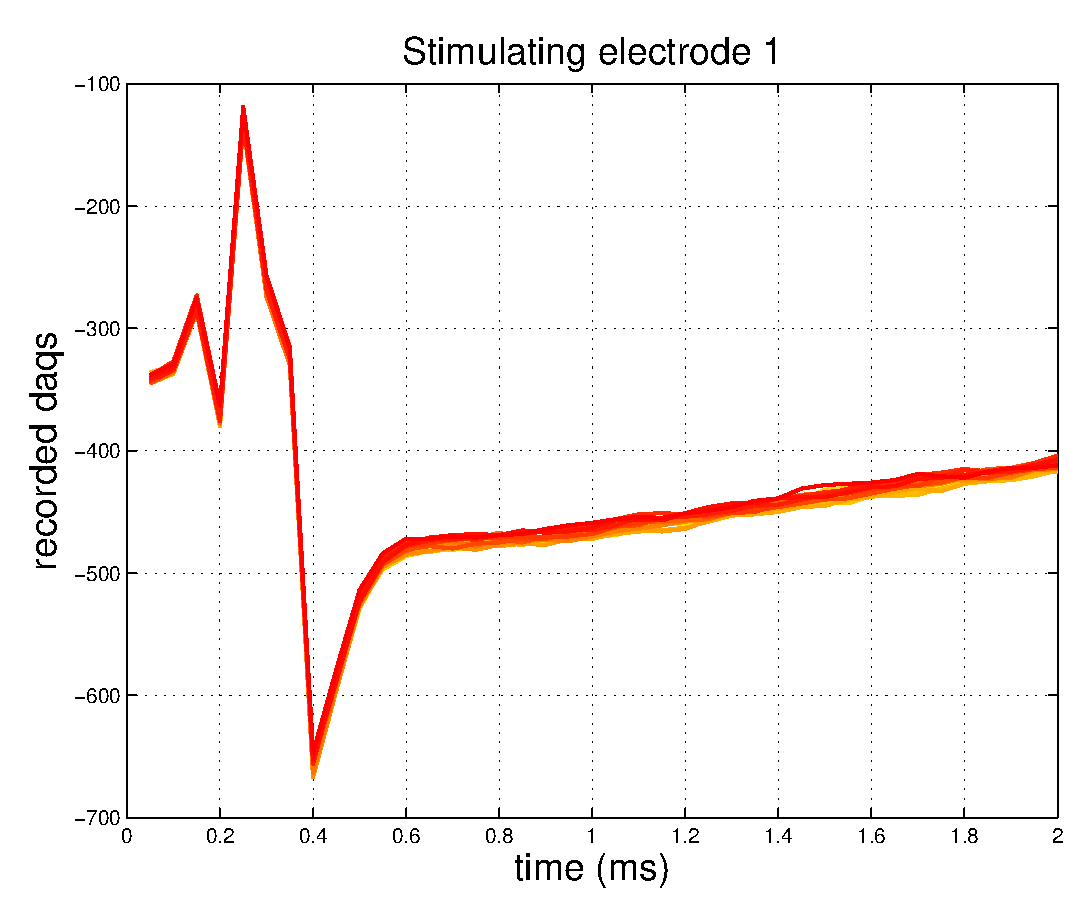
\includegraphics[width=\textwidth]{ArtTraceS1.eps}
                \caption{}
        \end{subfigure}% 
~\begin{subfigure}[b]{0.32\textwidth}
                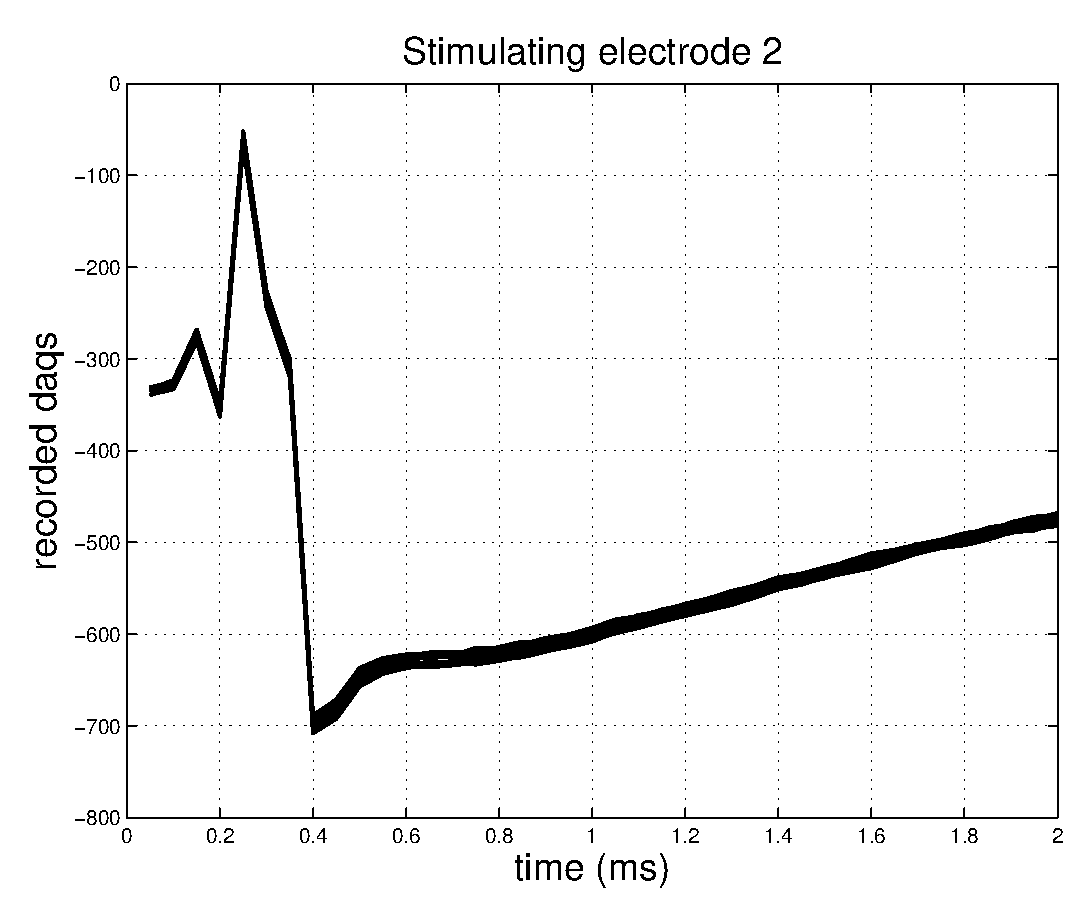
\includegraphics[width=\textwidth]{ArtTraceS2.eps}
                \caption{}
        \end{subfigure}
      ~  \begin{subfigure}[b]{0.32\textwidth}
                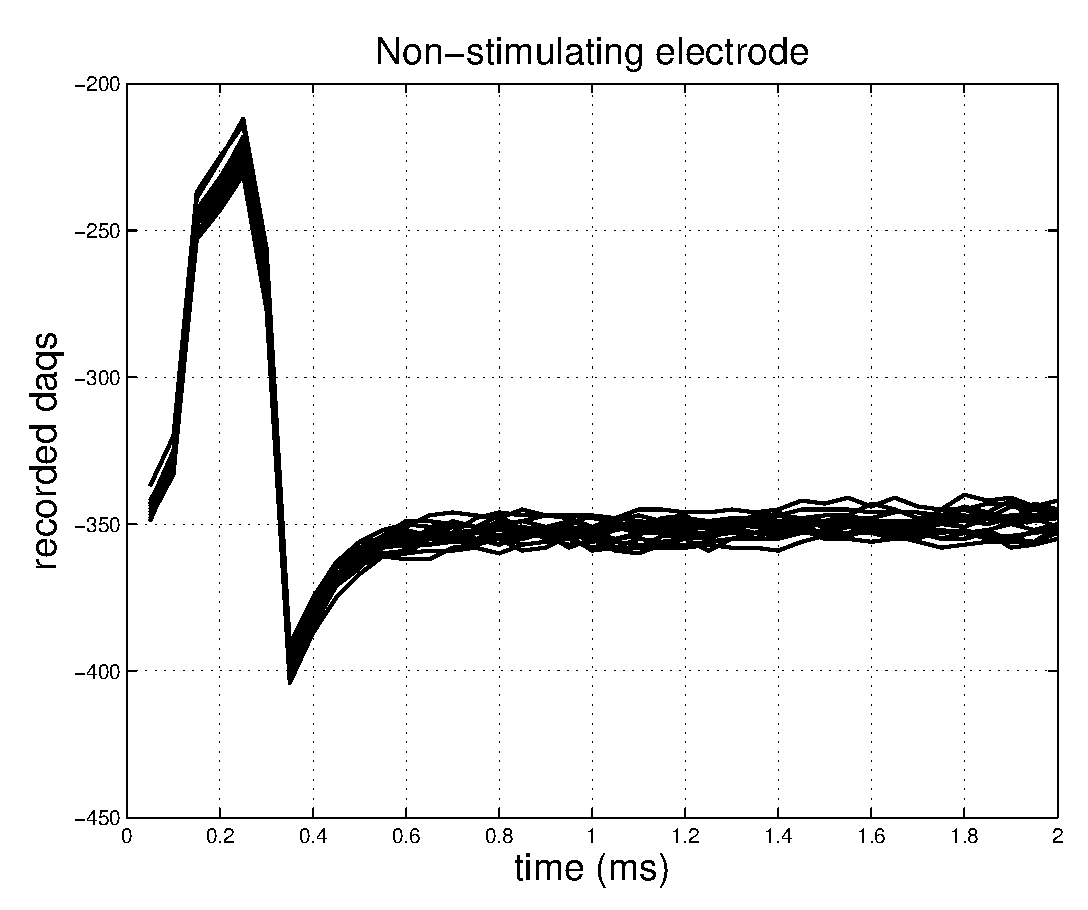
\includegraphics[width=\textwidth]{ArtTraceNS.eps}
                \caption{}
        \end{subfigure}
        \\
         \begin{subfigure}[b]{0.32\textwidth}
                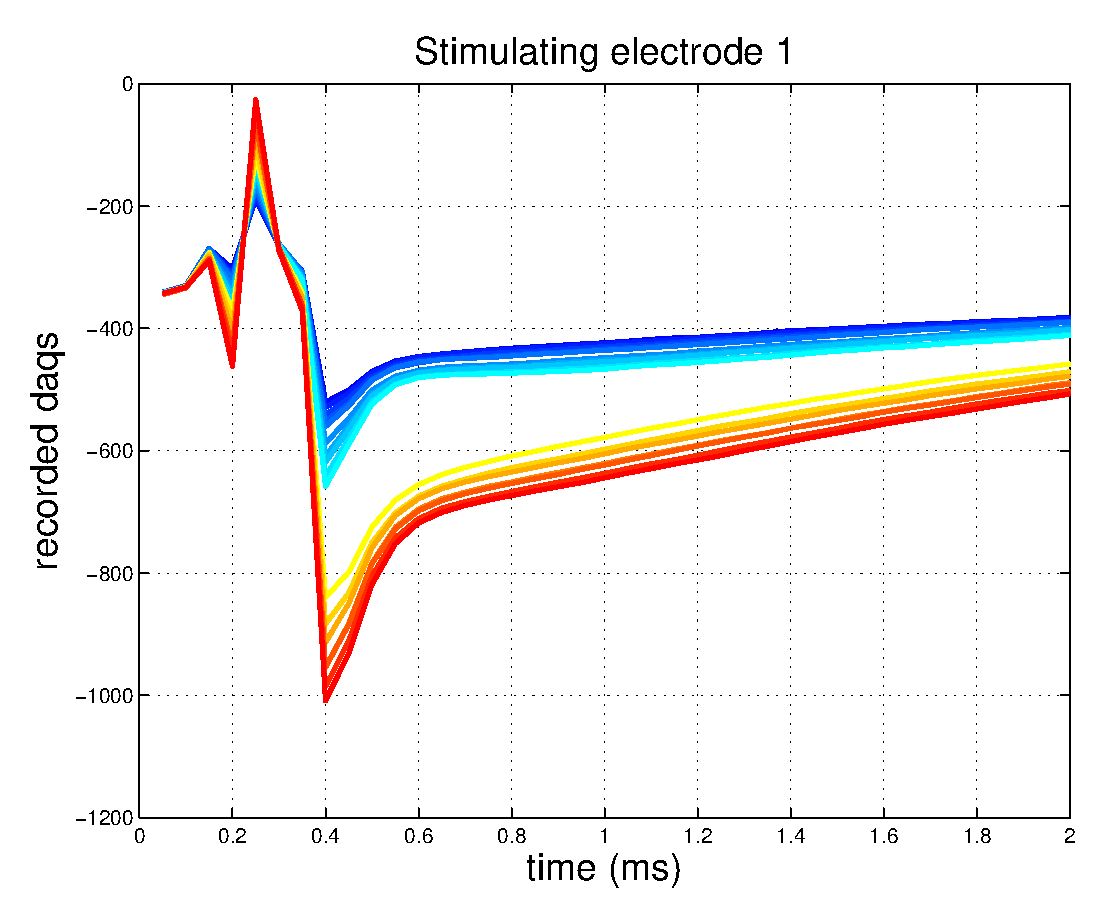
\includegraphics[width=\textwidth]{ArtMeanS1.eps}
                \caption{}
        \end{subfigure}     
       ~ \begin{subfigure}[b]{0.32\textwidth}
                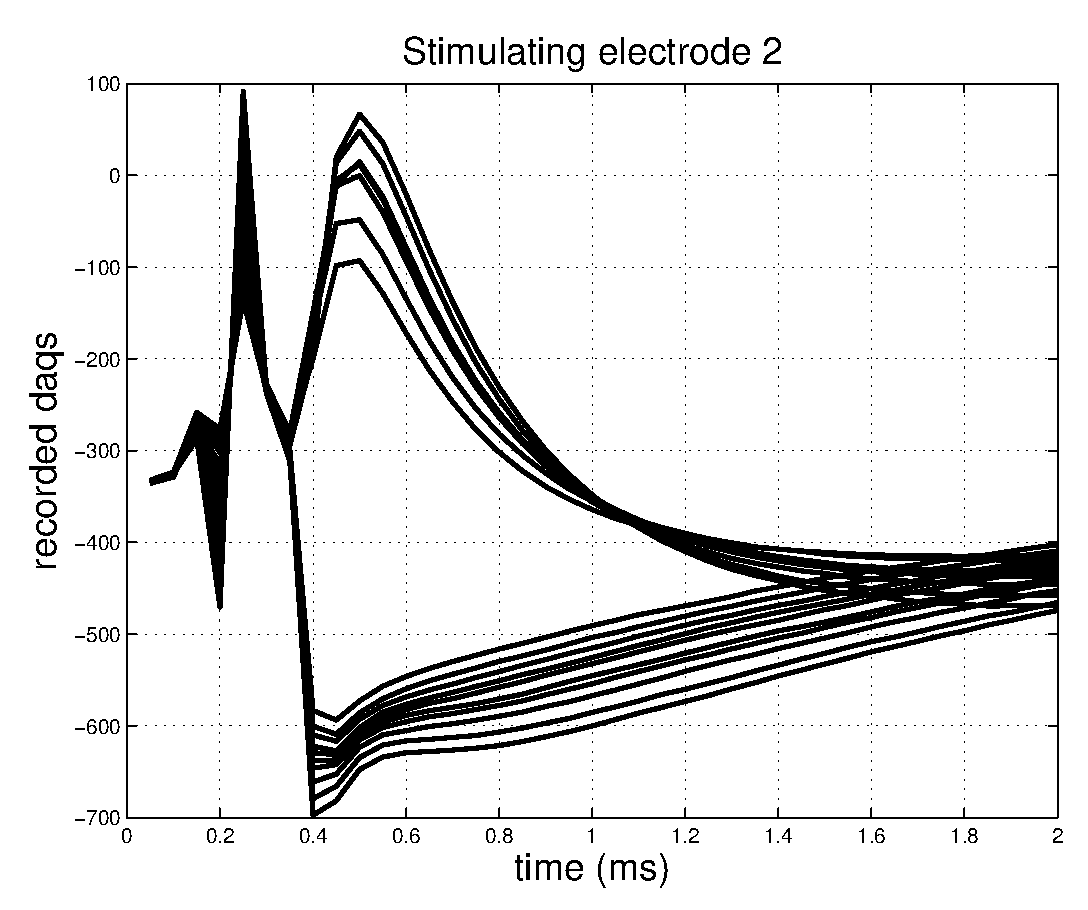
\includegraphics[width=\textwidth]{ArtMeanS2.eps}
                \caption{}
        \end{subfigure}
       ~ \begin{subfigure}[b]{0.32\textwidth}
                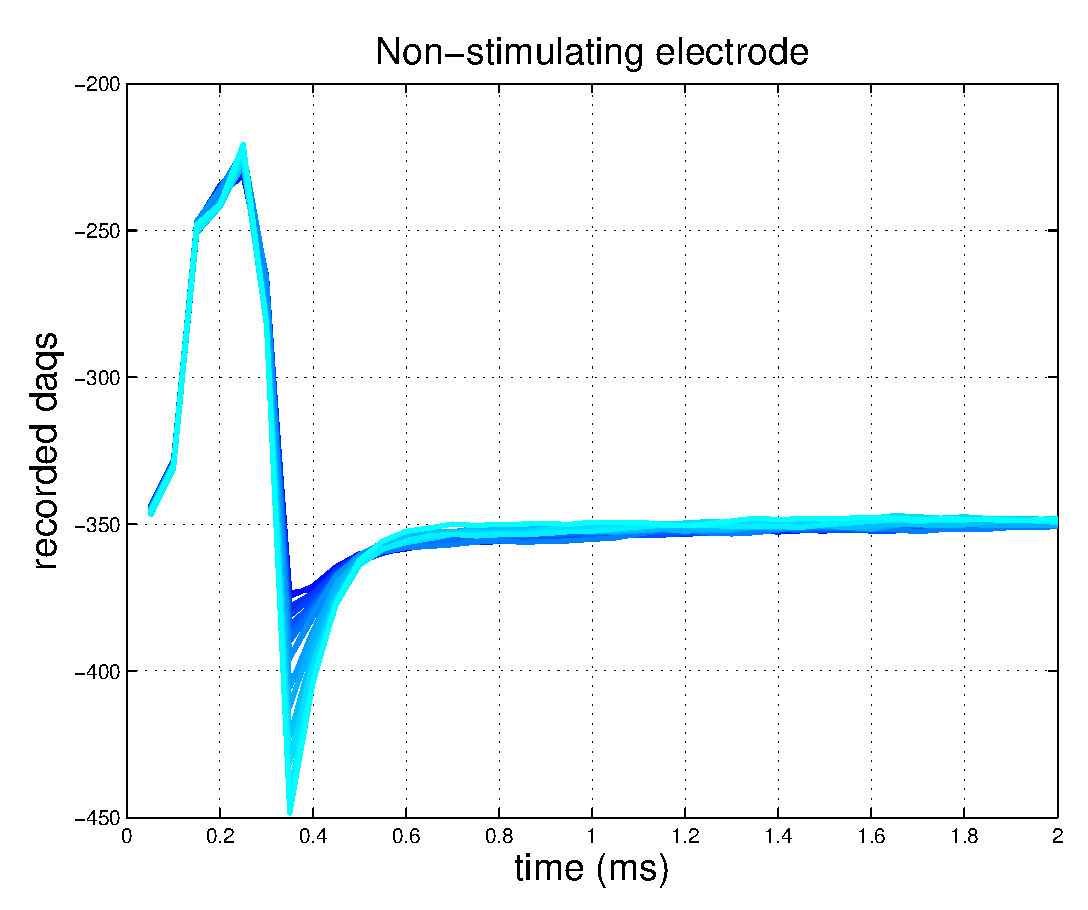
\includegraphics[width=\textwidth]{ArtMeansNS.eps}
                \caption{}

        \end{subfigure}
\caption{TTX experiments are useful to probe into the structure of hardware artifact. Current pulses were passed through two stimulating electrodes (current amplitudes between 0.5 and 2.3 mA) and responses were recorded in three electrodes.
 (a)-(c) Trial-by-trial variability in the artifact when stimulus is kept the same. Each colored line is a recorded trace recorded at different electrodes: in (a) and (b) they are the stimulating electrodes and (c) it is a non-recording, but neighboring electrode. (d)-(f). Artifact as a function of condition of stimulation. Each colored line is the artifact (average across trials) for a different condition. Light blue to blue are traces in the first inter-breakpoint range, and orange to red traces in the second. For the stimulating electrodes, (d) and (e), sensible changes are observed after a breakpoint, which makes extrapolation difficult. For the non-stimulating electrode (f) no discontinuities are observed. There is no clear pattern that explains condition and time variations in artifacts, but they all exhibit time smoothness (mostly after 0.6 ms), and condition smoothness for conditions in the same inter-breakpoint range.
}
\label{fig:ttx}
\end{figure}
\pagebreak

\begin{figure}[ht!]
        \centering
        \begin{subfigure}[b]{0.23\textwidth}
                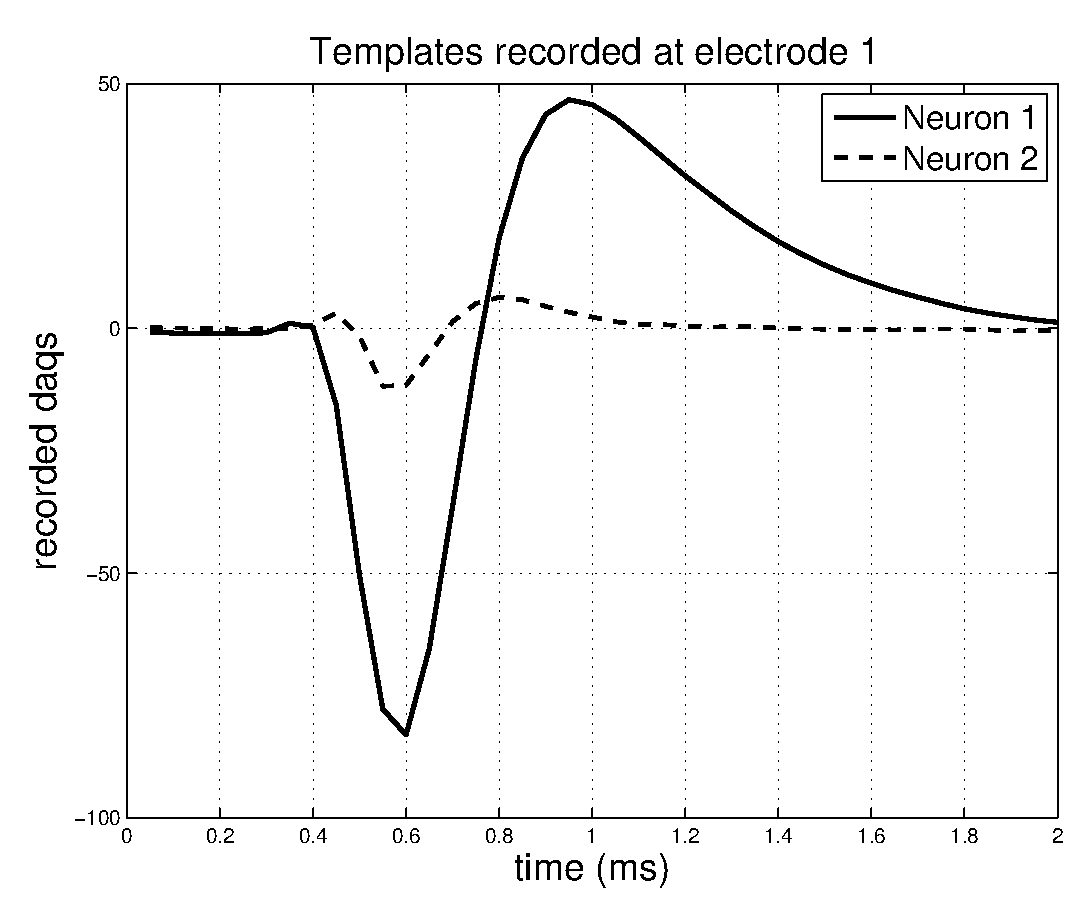
\includegraphics[width=\textwidth]{TemplateEL1.eps}
                \caption{}
        \end{subfigure}% 
~\begin{subfigure}[b]{0.23\textwidth}
                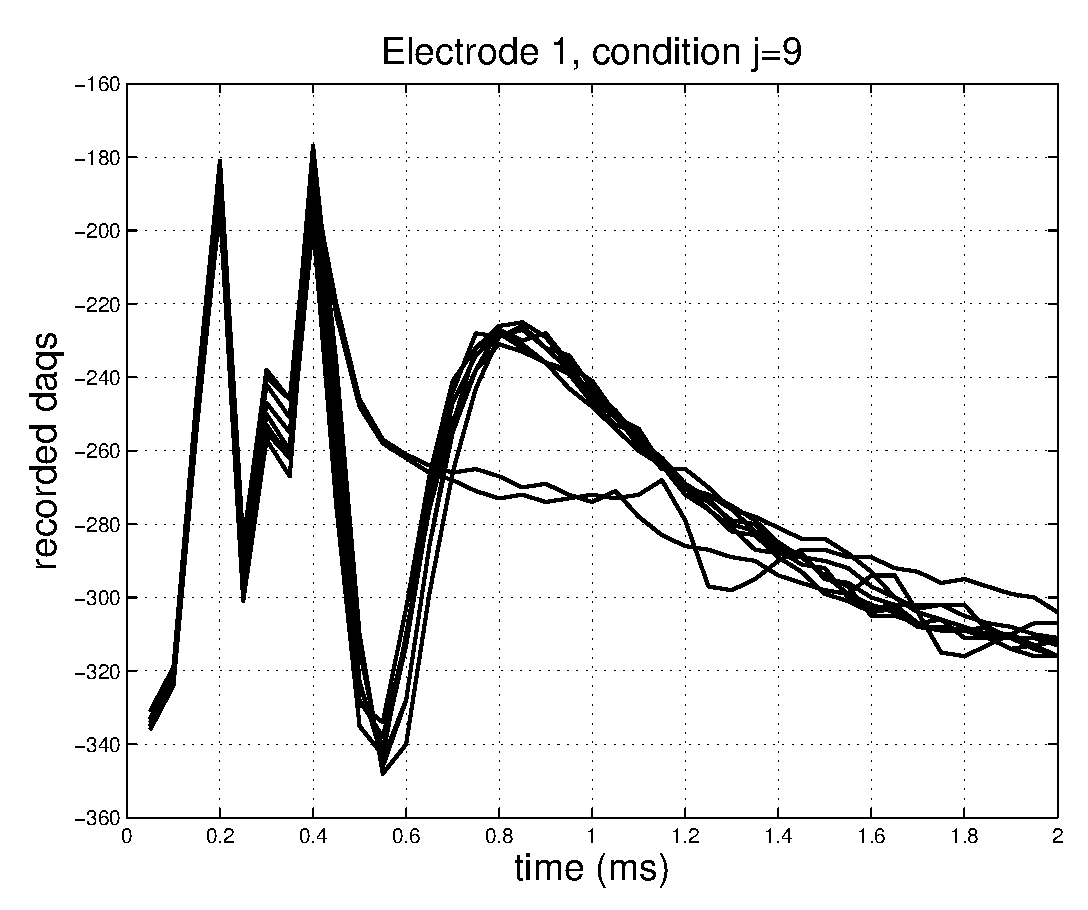
\includegraphics[width=\textwidth]{EL11.eps}
                \caption{}
        \end{subfigure}
      ~  \begin{subfigure}[b]{0.23\textwidth}
                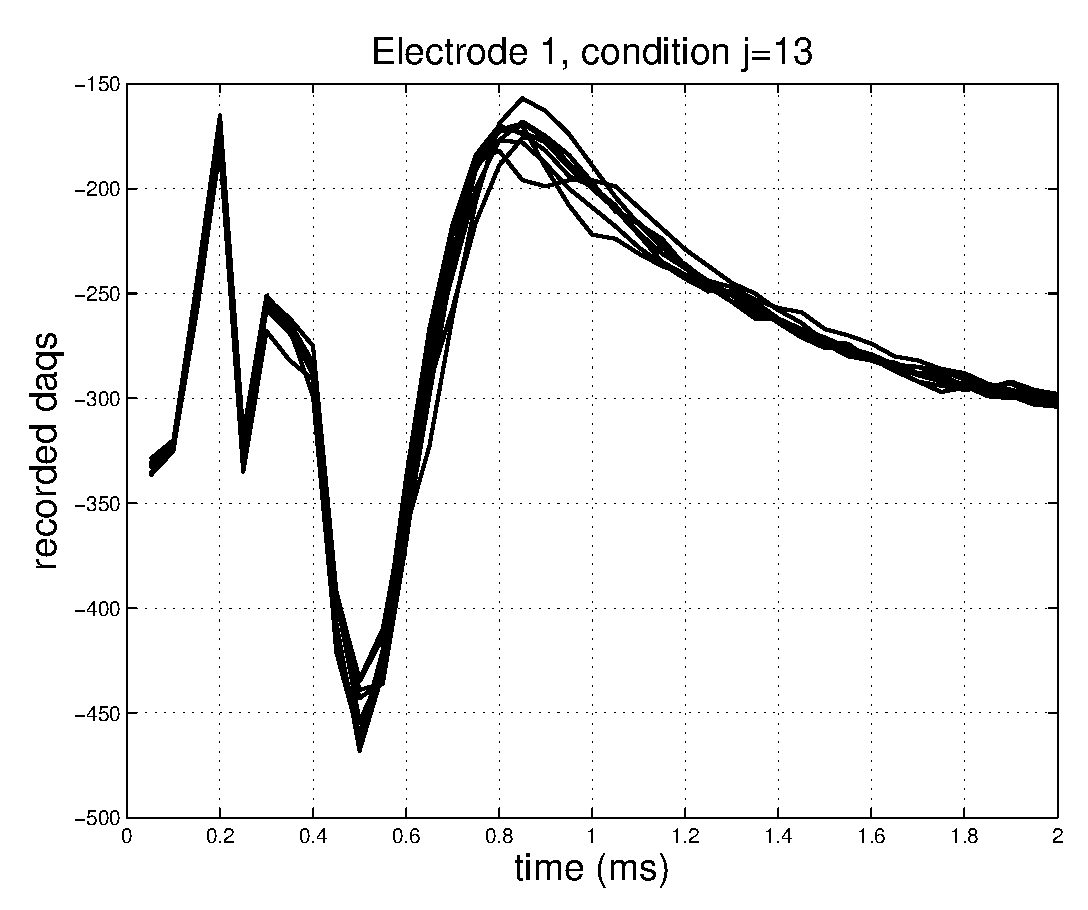
\includegraphics[width=\textwidth]{EL12.eps}
                \caption{}
        \end{subfigure}
        ~  \begin{subfigure}[b]{0.23\textwidth}
                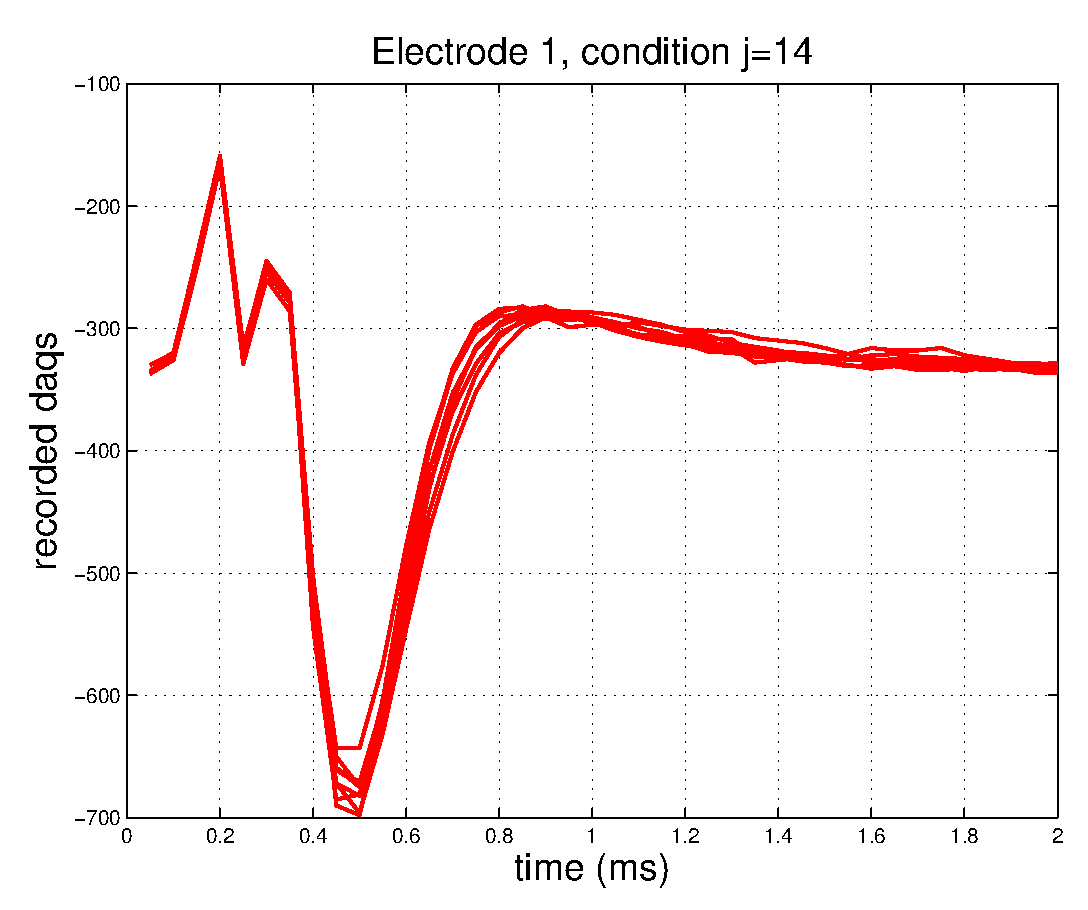
\includegraphics[width=\textwidth]{EL13.eps}
                \caption{}
        \end{subfigure}
        \\
         \begin{subfigure}[b]{0.23\textwidth}
                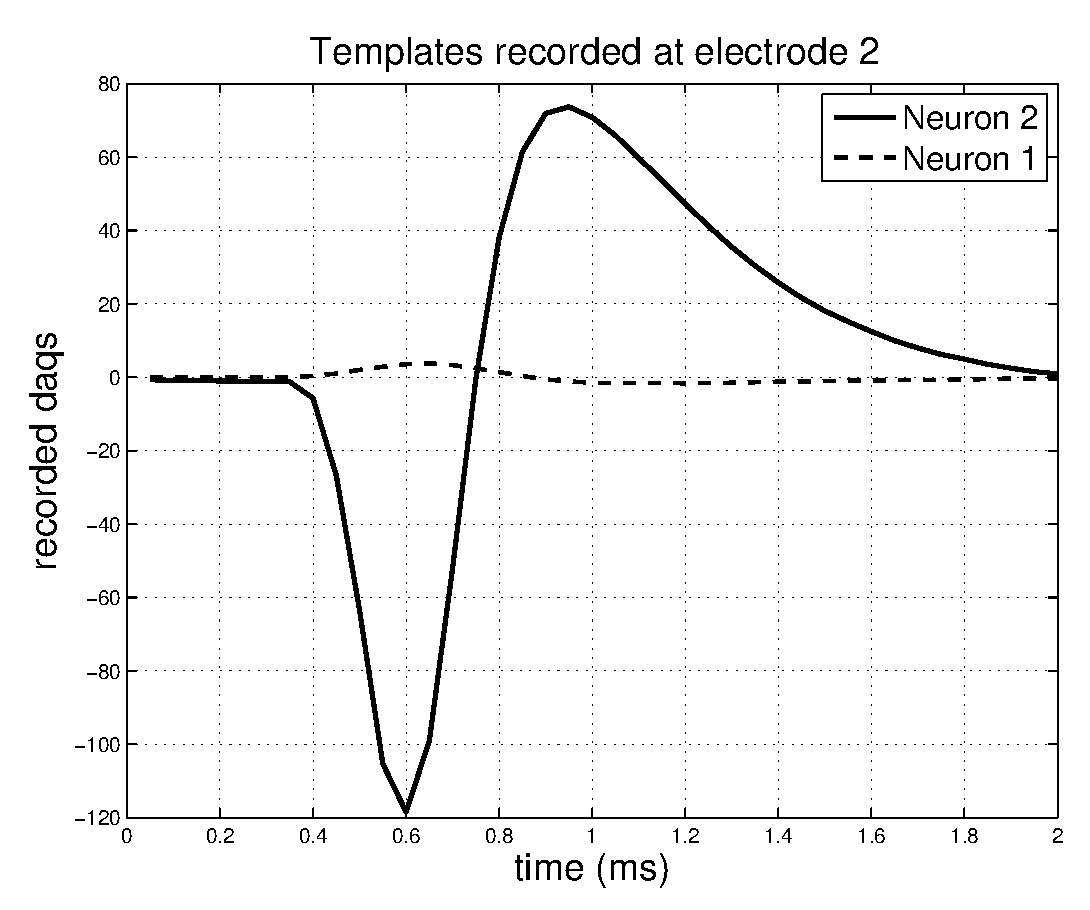
\includegraphics[width=\textwidth]{TemplateEL2.eps}
                \caption{}
        \end{subfigure}     
       ~ \begin{subfigure}[b]{0.23\textwidth}
                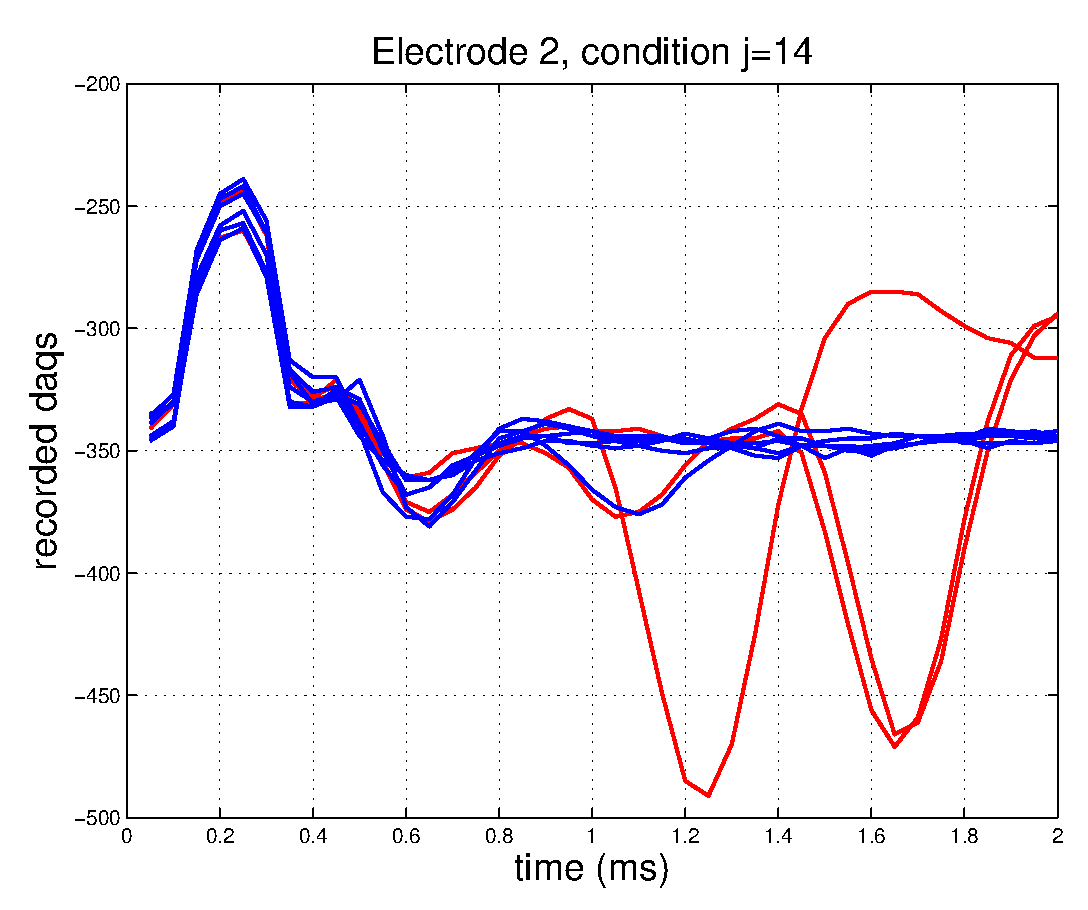
\includegraphics[width=\textwidth]{EL21.eps}
                \caption{}
        \end{subfigure}
       ~ \begin{subfigure}[b]{0.23\textwidth}
                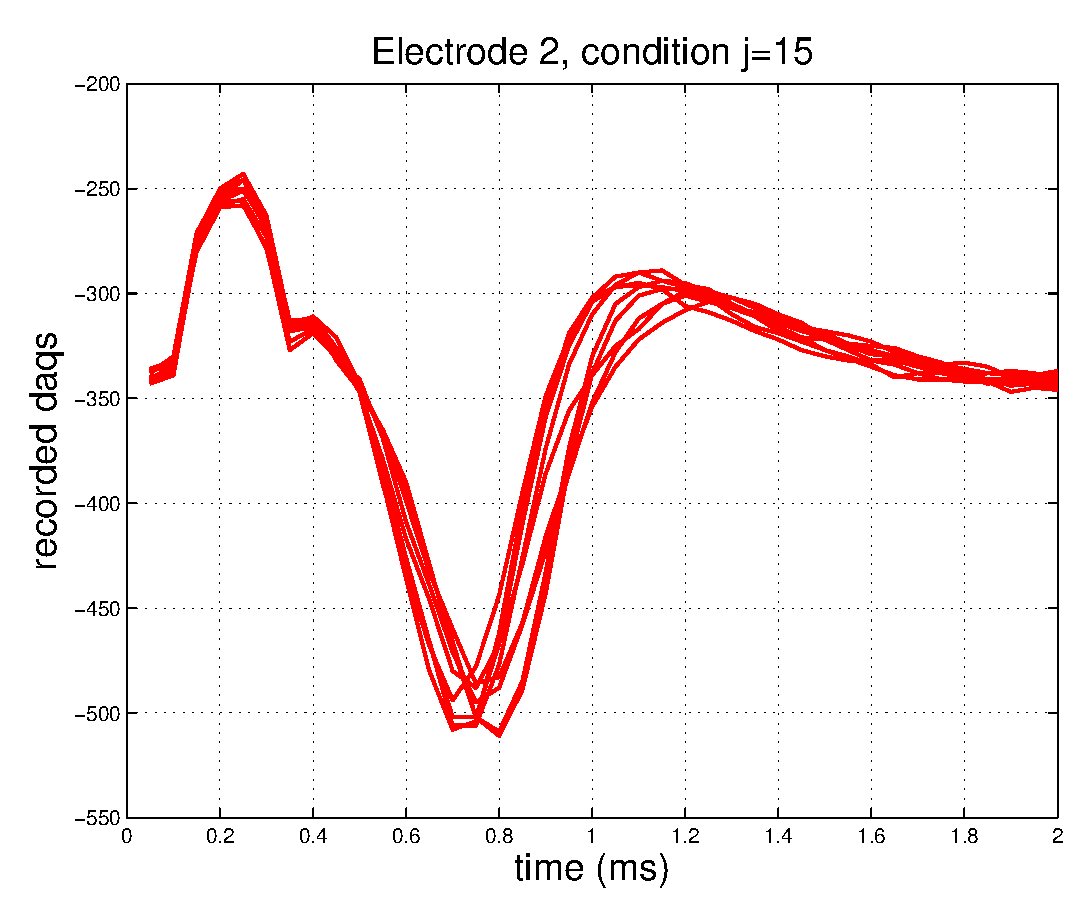
\includegraphics[width=\textwidth]{EL22.eps}
                \caption{}
                \end{subfigure}
~ \begin{subfigure}[b]{0.23\textwidth}
                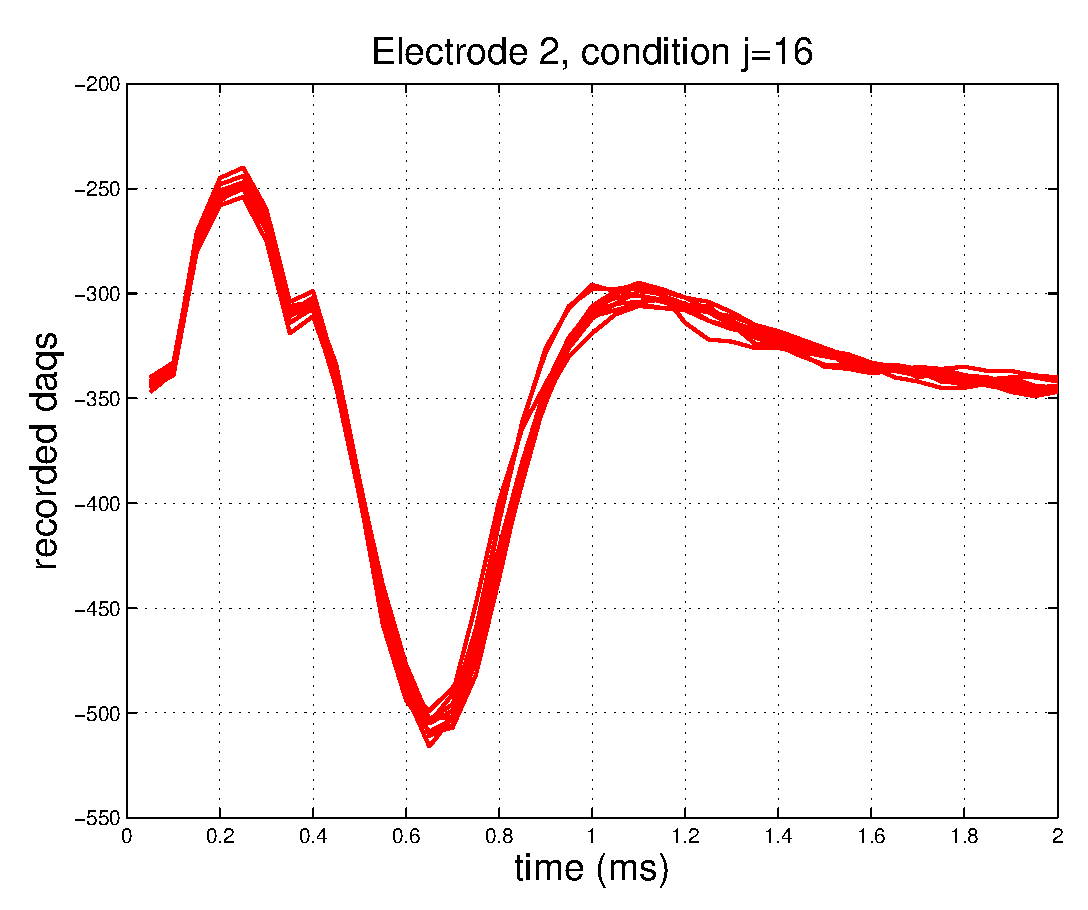
\includegraphics[width=\textwidth]{EL23.eps}
                \caption{}
        \end{subfigure}
\caption{Caption: Examples of recorded traces in a experiment with two stimulating electrodes and two neurons. In one of the stimulating electrodes (electrode 1) neuron 1 has a strong signal, as shown by templates in (a), and neuron 2 has a strong signal only in a non-stimulating electrode (electrode 2), as shown in (e).
(b)-(d) show all traces in electrode 1 for different conditions. Presence or absence of spiking is indicated by red or blue colors, respectively. In (b) spike sorting is straightforward by mere visual inspection of traces and template, which is no longer true for (c ) and (d). In (c) all trials have spikes, but notice voltage the deflection around t=0.6ms doesn?t match the template as in (b). The reason is that artifact also contributes to that deflection. Because of this, spike identification requires a more thorough treatment: for example, if a good guess of the artifact can be obtained by an extrapolation from previous conditions, then it can be subtracted for subsequent template matching with the residuals (not shown). However, that is not possible in (d), as condition 14 is the first following a breakpoint, making extrapolation senseless. The decision has to be made by an activation curve criterion: for their similarity all traces either have or don?t have spikes, but absence of spikes is unlikely because activation was observed at previous conditions. (f)-(h) show traces in electrode 2, and illustrate ubiquitous phenomena: First, notice in (f) there are traces with voltage deflections that are not explained by none of the two neurons. These are the result of transient changes in background activity, characteristic to each condition (for example, spiking of other neurons not relevant for spike sorting). This justifies the use of condition dependent residual variances. Second, notice variability in spike latencies decreases with condition until variability is barely noticeable. In this steady regime spike identification is hampered, as spike and artifact contributions to data are difficult to distinguish. }
\label{fig:traces}
\end{figure}
\pagebreak
\graphicspath{ {./FiguresMethods/AlgExample/} }
\begin{figure}[ht!]
        \centering
        \begin{subfigure}[b]{0.32\textwidth}
                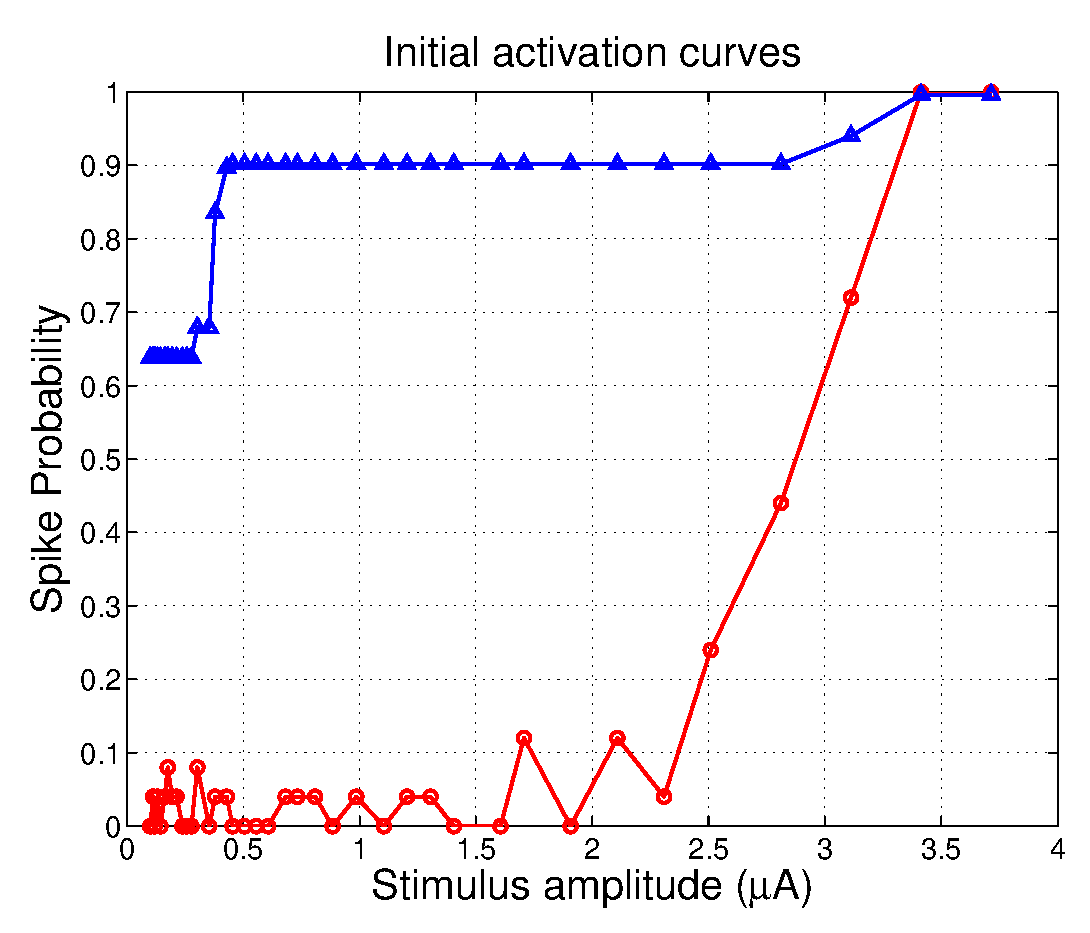
\includegraphics[width=\textwidth]{Act0.eps}
                \caption{}
        \end{subfigure}% 
~\begin{subfigure}[b]{0.32\textwidth}
                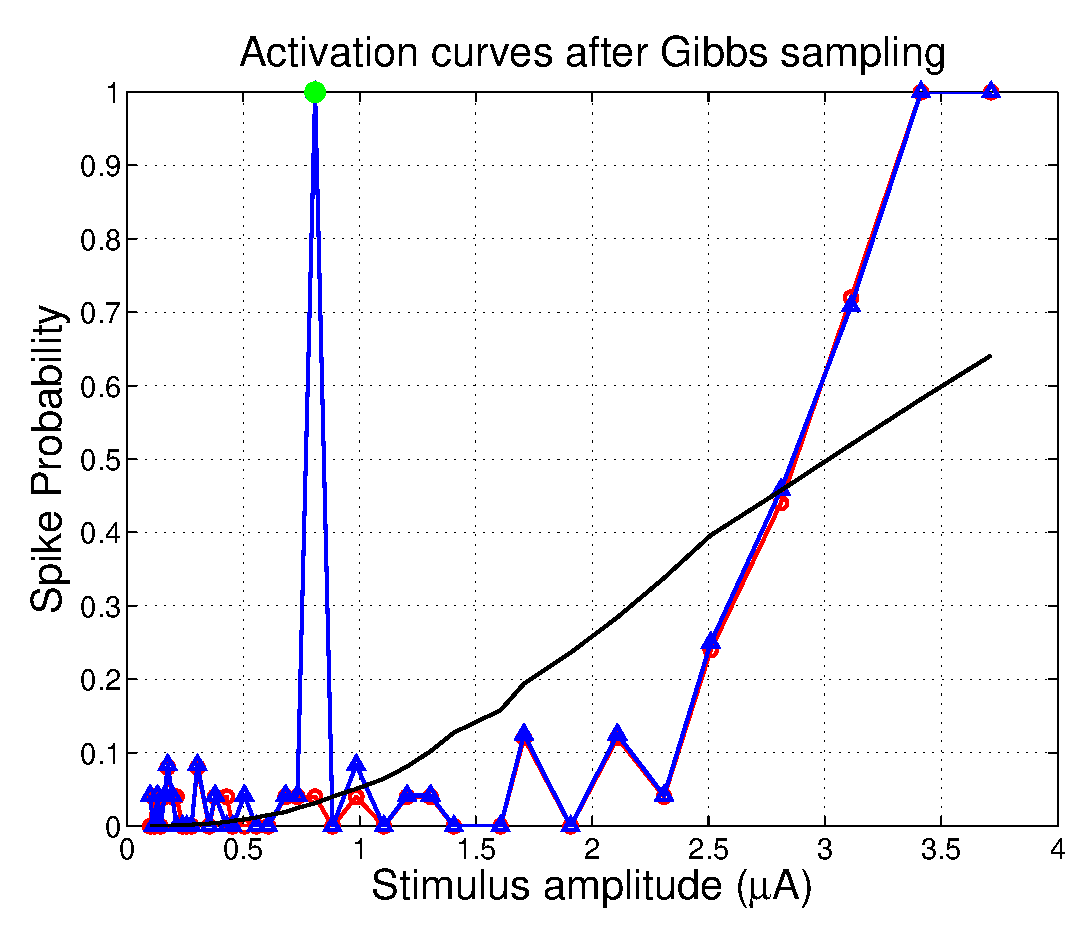
\includegraphics[width=\textwidth]{Act2.eps}
                \caption{}
        \end{subfigure}
      ~  \begin{subfigure}[b]{0.32\textwidth}
                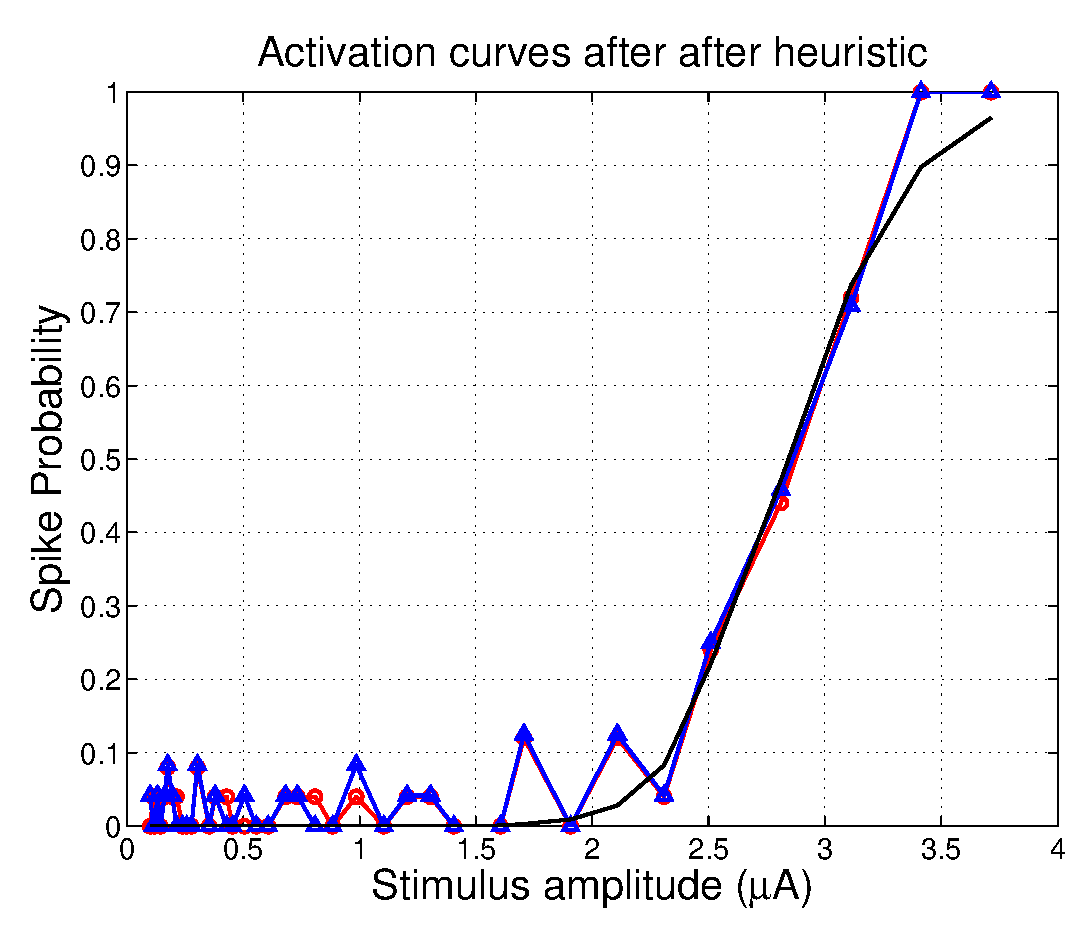
\includegraphics[width=\textwidth]{Act3.eps}
                \caption{}
        \end{subfigure}
        \\
         \begin{subfigure}[b]{0.32\textwidth}
                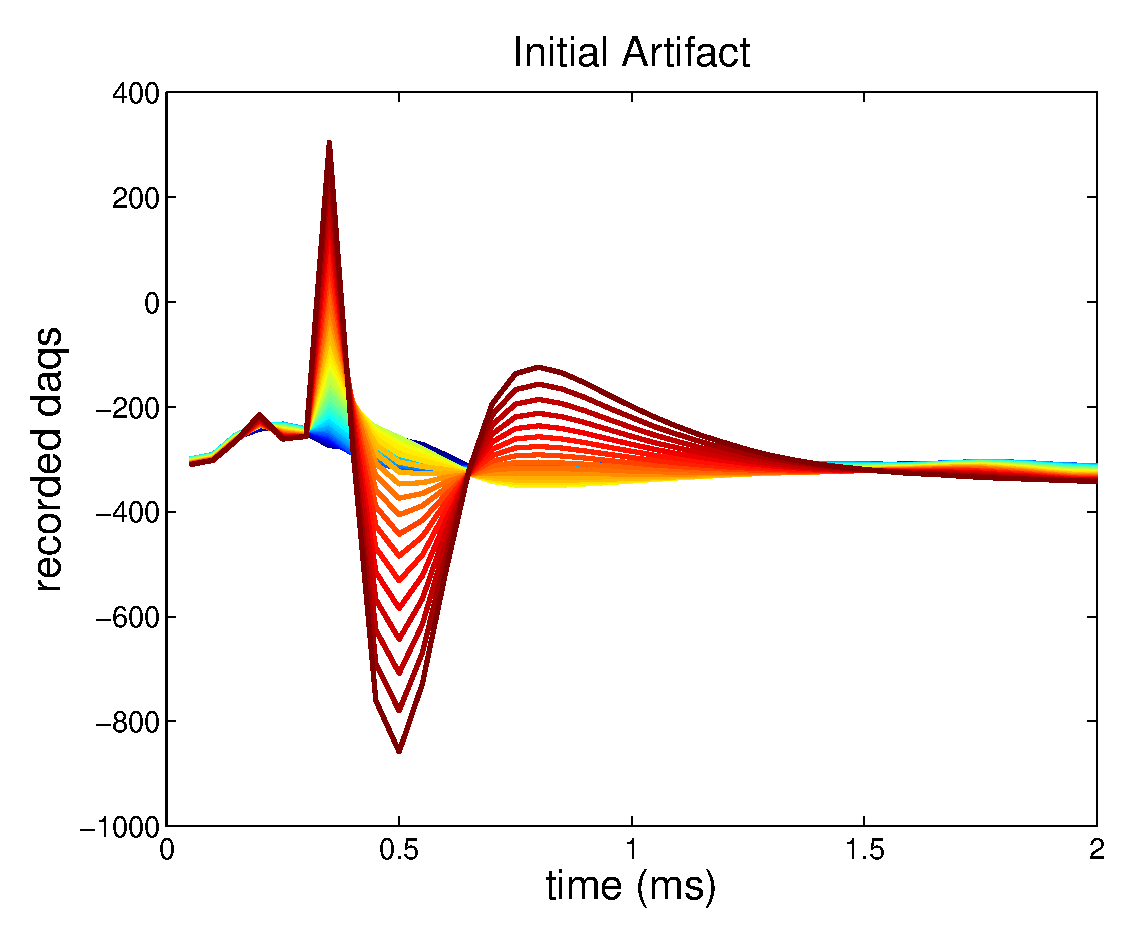
\includegraphics[width=\textwidth]{A0.eps}
                \caption{}
        \end{subfigure}     
       ~ \begin{subfigure}[b]{0.32\textwidth}
                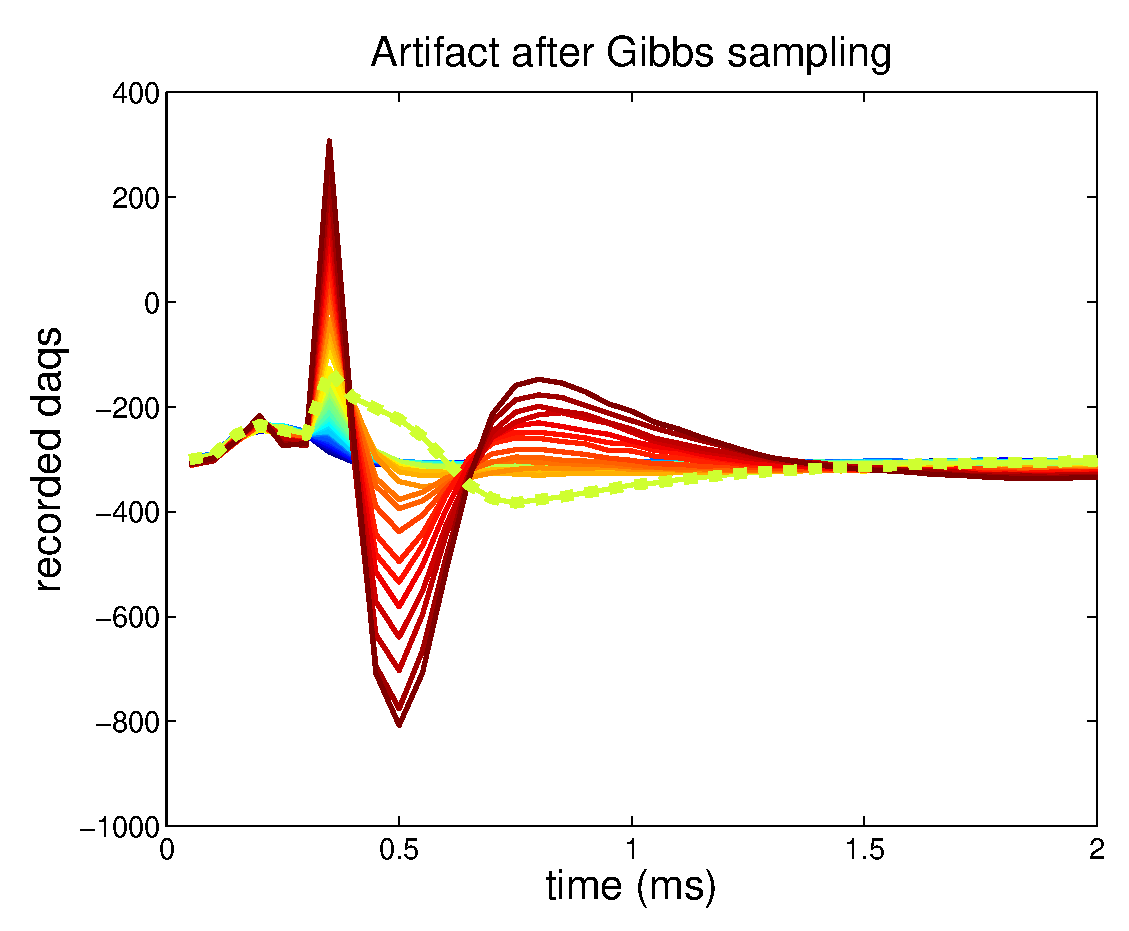
\includegraphics[width=\textwidth]{A2.eps}
                \caption{}
        \end{subfigure}
       ~ \begin{subfigure}[b]{0.32\textwidth}
                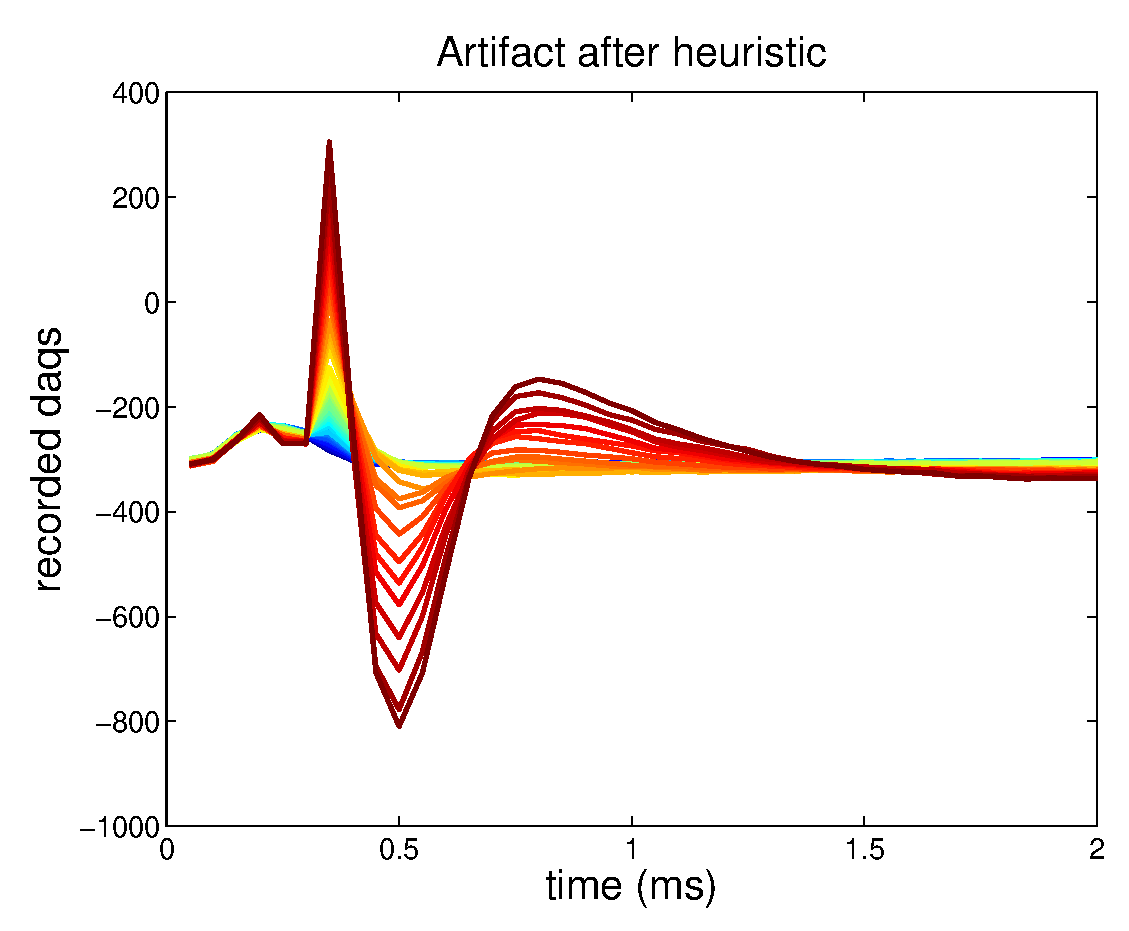
\includegraphics[width=\textwidth]{A3.eps}
                \caption{}
                \end{subfigure}
\caption{Example of the different stages of the algorithm. (a)-(c) Algorithm activation curves (blue traces) after initialization (a), first Gibbs sampling iteration (b) and heuristic post-processing (c ), along with ground truth activation curves (red traces) and logistic regression fit (black traces). (d)-(e) Artifact estimates at different stages of algorithm. Each colored trace corresponds to a different amplitude of stimulation (equivalently, conditions), with red traces representing high amplitudes. After the initialization the fit to ground truth is poor, although a useful polynomial estimate of the artifact is obtained. After Gibbs sampling the activation curves matches ground truth much better, but there is a condition where spikes are mistakenly inferred at all trials, denoted by the green circle in (b). This is diagnosed by a lack of fit with the underlying logistic regression, and prescribes the interpolation of the corresponding artifact, dashed line in (e), based in the information provided by the rest of non-dashed traces. As a result, a better estimate is obtained, spikes are no longer inferred at that condition, and lack of fit is no further diagnosed, leading to termination.}
\label{fig:traces}
\end{figure}

\graphicspath{ {././ResultsFigures/}}
\begin{figure}[ht!]
        \centering
        \begin{subfigure}[b]{0.5\textwidth}
                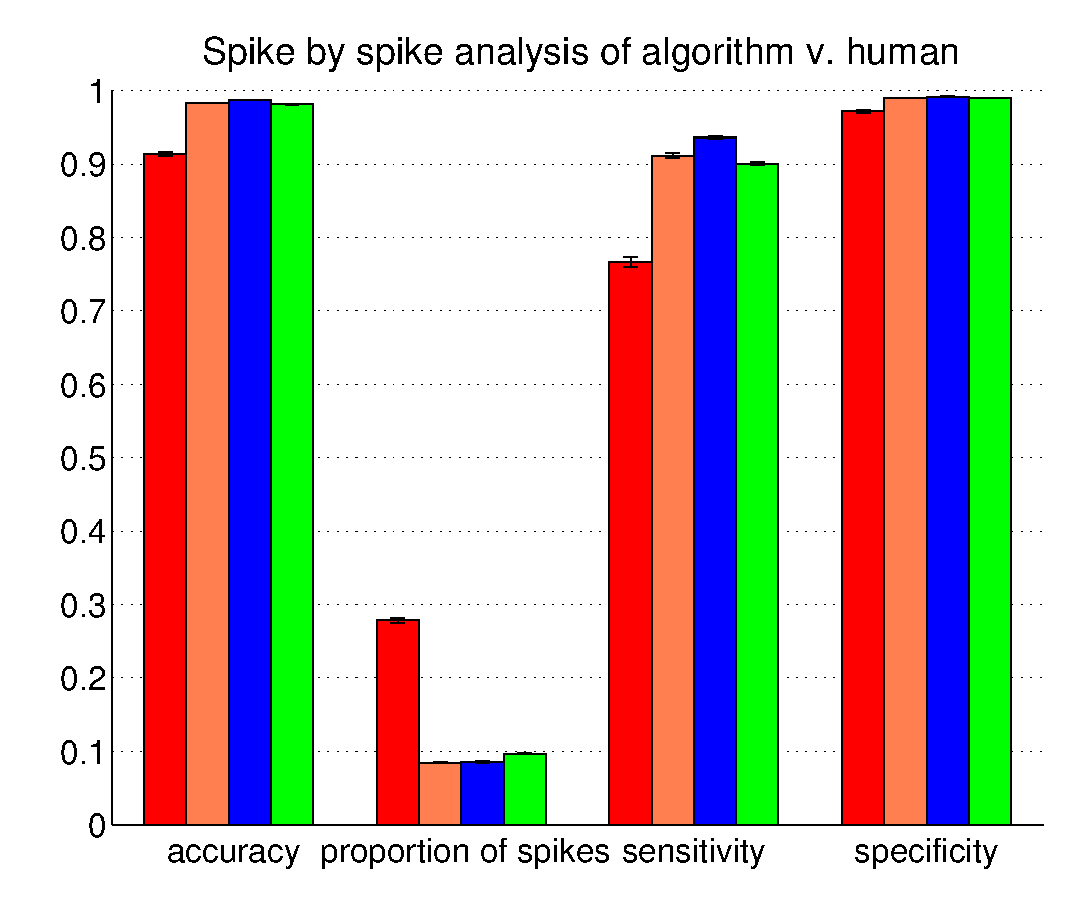
\includegraphics[width=\textwidth]{Barplots.eps}
                \caption{}
                \label{resultsOverall}
        \end{subfigure}% 
~\begin{subfigure}[b]{0.5\textwidth}
                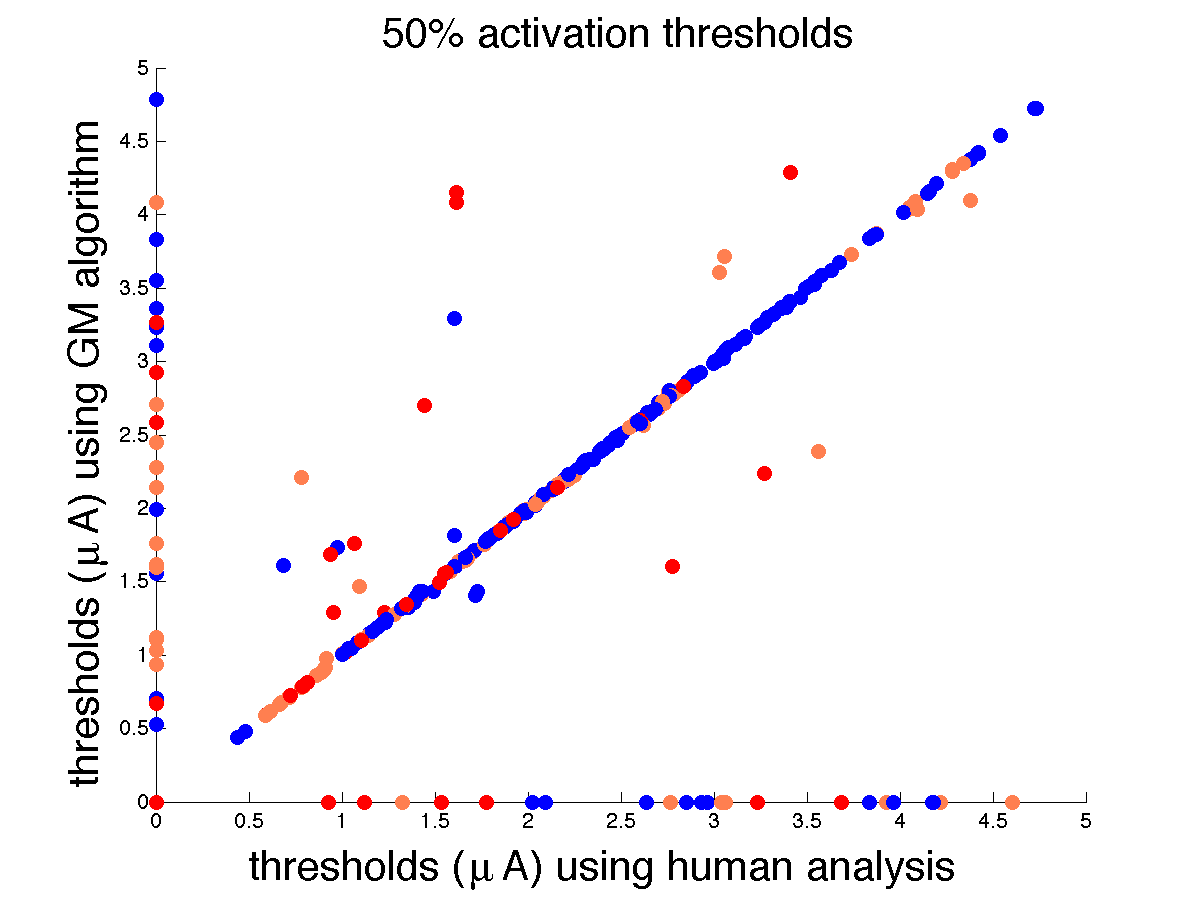
\includegraphics[width=\textwidth]{ScatterAll.eps}
                \caption{}
                \label{resultsScatter}
        \end{subfigure}
      \caption{(a) Bar plots representing performance measures for the three cases of recording-stimulating electrode relation, with red, orange and blue bars corresponding to (i), (ii), (iii) respectively. Green bars represent grand totals. (b) Scatterplot showing threshold comparisons, as an alternative measure to compare performance. Colors represent the same as in (a). True negatives are indicated by the dot at $(0,0)$ (many overlap), false positives by dots in the y-axis and false negatives by dots in the x-axis. The remaining dots are true positives, and discrepancies between algorithm and ground truth are represented by vertical distances between dots and the diagonal}
\end{figure}



\begin{figure}[ht!]
        \centering
        \begin{subfigure}[b]{0.8\textwidth}
                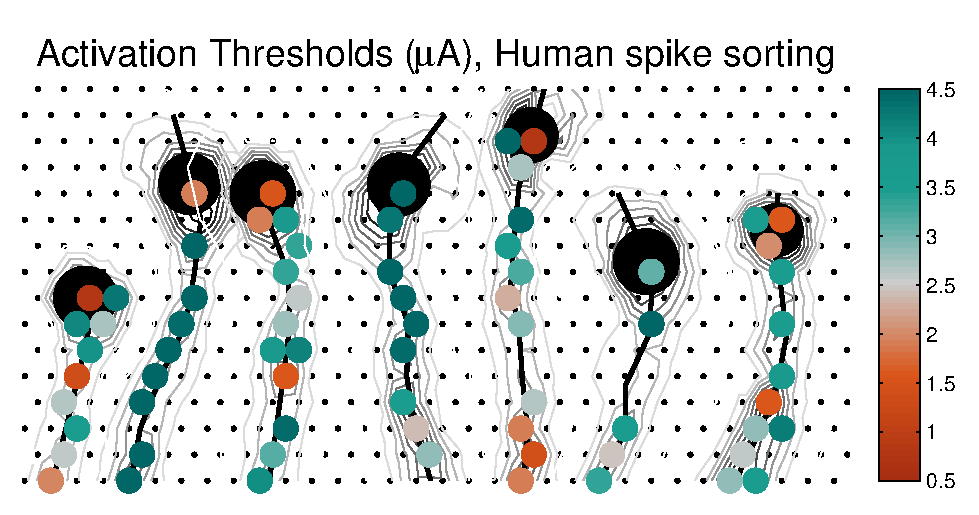
\includegraphics[width=\textwidth]{HumanActSeveralNeurons.eps}
                \caption{}
        \end{subfigure}% 
\\
\begin{subfigure}[b]{0.8\textwidth}
                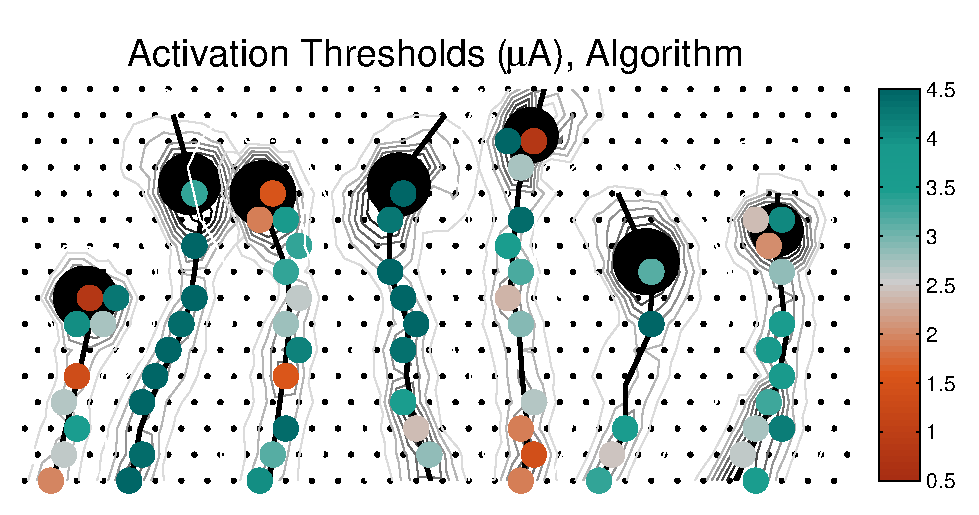
\includegraphics[width=\textwidth]{AlgActSeveralNeurons.eps}
                \caption{}
        \end{subfigure}
      \caption{An example of spatial sensitivity analysis: For the 7 cells targeted in the array the object is to determine which are the single stimulating electrodes that will trigger activation, and if that is the case, which is the activation threshold. In the figures, each small black dot is an electrode in the MEA and large dots are the electrodes for which activation was detected, based both in ground truth (a) or algorithm (b). Colors represent different activation thresholds.}
      \label{fig:spatialsens}
\end{figure}


\pagebreak

 \bibliographystyle{unsrt} 
\bibliography{references}


    \end{document}
